% Options for packages loaded elsewhere
\PassOptionsToPackage{unicode}{hyperref}
\PassOptionsToPackage{hyphens}{url}
%
\documentclass[
]{book}
\title{Plan Estadístico Institucional}
\author{ Universidad Nacional de Colombia Oficina Nacional de Estadística}
\date{}

\usepackage{amsmath,amssymb}
\usepackage{lmodern}
\usepackage{iftex}
\ifPDFTeX
  \usepackage[T1]{fontenc}
  \usepackage[utf8]{inputenc}
  \usepackage{textcomp} % provide euro and other symbols
\else % if luatex or xetex
  \usepackage{unicode-math}
  \defaultfontfeatures{Scale=MatchLowercase}
  \defaultfontfeatures[\rmfamily]{Ligatures=TeX,Scale=1}
\fi
% Use upquote if available, for straight quotes in verbatim environments
\IfFileExists{upquote.sty}{\usepackage{upquote}}{}
\IfFileExists{microtype.sty}{% use microtype if available
  \usepackage[]{microtype}
  \UseMicrotypeSet[protrusion]{basicmath} % disable protrusion for tt fonts
}{}
\makeatletter
\@ifundefined{KOMAClassName}{% if non-KOMA class
  \IfFileExists{parskip.sty}{%
    \usepackage{parskip}
  }{% else
    \setlength{\parindent}{0pt}
    \setlength{\parskip}{6pt plus 2pt minus 1pt}}
}{% if KOMA class
  \KOMAoptions{parskip=half}}
\makeatother
\usepackage{xcolor}
\IfFileExists{xurl.sty}{\usepackage{xurl}}{} % add URL line breaks if available
\IfFileExists{bookmark.sty}{\usepackage{bookmark}}{\usepackage{hyperref}}
\hypersetup{
  pdftitle={Plan Estadístico Institucional},
  pdfauthor={ Universidad Nacional de Colombia   Oficina Nacional de Estadística},
  hidelinks,
  pdfcreator={LaTeX via pandoc}}
\urlstyle{same} % disable monospaced font for URLs
\usepackage{longtable,booktabs,array}
\usepackage{calc} % for calculating minipage widths
% Correct order of tables after \paragraph or \subparagraph
\usepackage{etoolbox}
\makeatletter
\patchcmd\longtable{\par}{\if@noskipsec\mbox{}\fi\par}{}{}
\makeatother
% Allow footnotes in longtable head/foot
\IfFileExists{footnotehyper.sty}{\usepackage{footnotehyper}}{\usepackage{footnote}}
\makesavenoteenv{longtable}
\usepackage{graphicx}
\makeatletter
\def\maxwidth{\ifdim\Gin@nat@width>\linewidth\linewidth\else\Gin@nat@width\fi}
\def\maxheight{\ifdim\Gin@nat@height>\textheight\textheight\else\Gin@nat@height\fi}
\makeatother
% Scale images if necessary, so that they will not overflow the page
% margins by default, and it is still possible to overwrite the defaults
% using explicit options in \includegraphics[width, height, ...]{}
\setkeys{Gin}{width=\maxwidth,height=\maxheight,keepaspectratio}
% Set default figure placement to htbp
\makeatletter
\def\fps@figure{htbp}
\makeatother
\setlength{\emergencystretch}{3em} % prevent overfull lines
\providecommand{\tightlist}{%
  \setlength{\itemsep}{0pt}\setlength{\parskip}{0pt}}
\setcounter{secnumdepth}{5}
\newlength{\cslhangindent}
\setlength{\cslhangindent}{1.5em}
\newlength{\csllabelwidth}
\setlength{\csllabelwidth}{3em}
\newlength{\cslentryspacingunit} % times entry-spacing
\setlength{\cslentryspacingunit}{\parskip}
\newenvironment{CSLReferences}[2] % #1 hanging-ident, #2 entry spacing
 {% don't indent paragraphs
  \setlength{\parindent}{0pt}
  % turn on hanging indent if param 1 is 1
  \ifodd #1
  \let\oldpar\par
  \def\par{\hangindent=\cslhangindent\oldpar}
  \fi
  % set entry spacing
  \setlength{\parskip}{#2\cslentryspacingunit}
 }%
 {}
\usepackage{calc}
\newcommand{\CSLBlock}[1]{#1\hfill\break}
\newcommand{\CSLLeftMargin}[1]{\parbox[t]{\csllabelwidth}{#1}}
\newcommand{\CSLRightInline}[1]{\parbox[t]{\linewidth - \csllabelwidth}{#1}\break}
\newcommand{\CSLIndent}[1]{\hspace{\cslhangindent}#1}
\usepackage{booktabs}
\usepackage{float}
\usepackage[left=3cm,right=3cm,top=6cm,bottom=6cm]{geometry}
\ifxetex
  \usepackage{polyglossia}
  \setmainlanguage{spanish}
  % Tabla en lugar de cuadro
  \gappto\captionsspanish{\renewcommand{\tablename}{Tabla}  
          \renewcommand{\listtablename}{Índice de tablas}}
\else
  \usepackage[spanish,es-tabla]{babel}
\fi
\ifLuaTeX
  \usepackage{selnolig}  % disable illegal ligatures
\fi

\begin{document}
\maketitle

{
\setcounter{tocdepth}{1}
\tableofcontents
}
\hypertarget{portada}{%
\chapter*{Portada}\label{portada}}
\addcontentsline{toc}{chapter}{Portada}

\begin{center}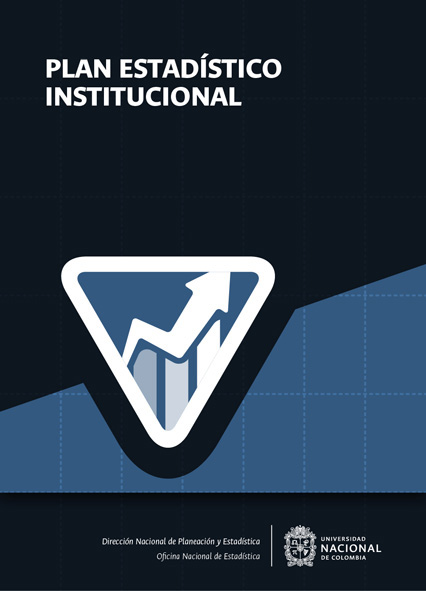
\includegraphics[width=0.75\linewidth]{Imagenes/Portada Final} \end{center}

\hypertarget{intro}{%
\chapter{Introducción}\label{intro}}

La Universidad Nacional de Colombia (UNAL), ente rector de la educación superior de Colombia, consciente de la necesidad de fortalecer los procesos de producción y difusión de la información estadística, así como de responder de una manera más adecuada a los requerimientos de información de la academia, las instituciones nacionales e internacionales, la comunidad universitaria y de la propia entidad, y considerando que la poca visibilización de la información es uno de los puntos neurálgicos de la gestión pública, ha tomado la iniciativa de formular un Plan Estadístico Institucional.

Este ejercicio se soporta conceptualmente de los lineamientos metodológicos del Departamento Administrativo Nacional de Estadistica, DANE, que según el decreto 4178 de 2012 tiene entre sus funciones la planificación, estandarización y certificación de las estadísticas. Parafraseando al \protect\hyperlink{ref-BibEntry2021Apr}{{``{DANE}''}} (\protect\hyperlink{ref-BibEntry2021Apr}{2021}), un Plan Estadístico institucional es un instrumento de determinación y priorización de la información estadística y demás resultados que se requieren o desean generar en un ámbito institucional; éste contiene la información estratégica que se requiere para la formulación de políticas públicas, la planeación, la toma de decisiones, así como para la evaluación y el seguimiento a los planes misionales y de acción.

Es así como en el marco del proyecto del Fortalecimiento Estadístico de la Universidad - fase I y bajo la orientación de la Dirección Nacional de Planeación y Estadística, se busca visibilizar la información institucional generada - oferta -, evaluar los niveles de satisfacción de información demandada por las dependencias del nivel nacional e identificar los procesos de gestión de la información.

Este ejercicio de planificación estadística obedece a la necesidad de definir, organizar y priorizar la información estadística que requiere la Universidad, en función de solucionar los problemas de desconocimiento y baja utilización de la información producida, entre otros factores que configuran un tratamiento inadecuado de la información generada por las diferentes dependencias que componen la Universidad.

En consecuencia, la elaboración de un Plan Estadístico institucional para la UNAL, se constituye en una estrategia tanto para facilitar los procesos de toma de decisiones como para hacer más efectivos los mecanismos de rendición de cuentas a la ciudadanía, a partir de un mayor y mejor aprovechamiento de la información generada, avanzando con ello en el fortalecimiento de la transparencia, la honestidad y el control social efectivo e incluyente sobre la gestión adelantada.

Como este instrumento, se espera lograr reducir los requerimientos no satisfechos de información que se presentan en la Universidad, por lo menos en los que respecta al componente estratégico de la información estadística, en la medida en que se definirán las estadísticas que son prioritarias para dar cuenta del que hacer de la entidad en relación con los componentes de Investigación, Extensión, Admisión y Movilidad, entre otros.

El documentos que se presenta a continuación está conformado por la descripción de la metodología para elaborar el Plan Estadístico de la UNAL; el diagnóstico de la actividad estadística en la Universidad, según cada uno de los ejes temáticos de información estadística; los resultados del cruce de oferta y demanda de información estadística en la UNAL; la formulación de la parte estratégica del Plan Estadístico UNAL, el Plan de Acción Institucional y, por último, los anexos correspondientes a los metadatos de las operaciones estadísticas que resumen la oferta de estadísticas estratégicas de la UNAL. El inventario de información se construyó conjuntamente con los delegados de las áreas y dependencias entre los meses de octubre de 2016 y julio de 2017.

\hypertarget{el-plan-estaduxedstico}{%
\chapter{El Plan Estadístico}\label{el-plan-estaduxedstico}}

El Plan Estadístico es básicamente una herramienta que identifica, organiza, depura, prioriza y difunde la información estratégica que se requiere para la formulación de políticas, la planeación y
toma de decisiones, y para la evaluación y seguimiento a los procesos y procedimientos. Teniendo
en cuenta esta definición, el objetivo del presente plan es entonces \emph{``organizar los procesos de producción y de gestión de la información estadística de la entidad, de modo que se constituya en un soporte eficiente para la formulación de políticas públicas, la planeación, la toma de decisiones, el seguimiento y la evaluación de los planes misionales''}.

El plan tiene como uno de sus productos principales la generación de un inventario de
información, que contiene las fichas técnicas de las operaciones estadísticas, es decir, la
caracterización de los procesos en los cuales existe una captura de datos, procesamiento y análisis,
y generación información estadística (agregados estadísticos o indicadores). Se asume que la
información estadística es el conjunto de resultados cuantitativos que se obtienen mediante el
tratamiento sistemático de datos que se originan en encuestas, censos o mediante la
consolidación de registros, para la medición y estudio de fenómenos de interés. Los datos son las
unidades de información que incluyen percepciones, números, observaciones, hechos y cifras,
pero que al estar desligadas de un contexto particular carecen de sentido informativo.

La necesidad de contar con una herramienta que permitiera regular la producción y el uso de la
información estadística para su mejor aprovechamiento, y que además posibilite la coordinación y
participación de productores y usuarios, ha llevado a varios países e instituciones a desarrollar
planes estadísticos por su utilidad en cuanto a reducir requerimientos estadísticos, y aportar a la
organización y articulación de sistemas de información. Los planes estadísticos, en general, han sido adoptados e implementados con
mayor fuerza en la Unión Europea y la Comunidad Andina.

El Plan Estadístico Nacional de España ha sido el de mayor reconocimiento por su continuidad y
continuo crecimiento desde el año 2009, estando actualmente vinculado al Real Decreto
1017/2013, de 20 de diciembre para su cumplimiento y regulación, por el que se aprueba el Programa anual 2014 del Plan Estadístico Nacional 2013-2016. De igual manera, otras comunidades
de España como Cataluña y Andalucía y países de América como México, Uruguay, Perú, Chile
y Colombia han implementado planes estadísticos Nacionales.

A nivel Nacional, se han implementado planes en las corporaciones regionales de Cundinamarca,
Antioquia, Norte de Santander, Boyacá y Bucaramanga. Otras instituciones que los han
implementado son la Policía Nacional de Colombia, la Superintendencia de la Economía Solidaria,
el Consejo Superior de la Judicatura, Coldeportes, y finalmente el Plan Estadístico Nacional, como
parte de las acciones definidas por el SEN (Sistema Estadístico Nacional) todos ellos con la asesoría
técnica o elaboración directa del DANE.

En el año 2001, el DANE desarrolló una metodología para la planificación estadística, actualizada
en el 2007, que responde a las necesidades planteadas por los territorios, sectores y entes
gubernamentales frente a la organización y manejo de la información disponible para la toma de
decisiones y la formulación de planes y proyectos de desarrollo. Esta metodología es la guía para la
formulación del Plan Estadístico institucional de la Universidad Nacional de Colombia. No obstante,
como resultado de las mesas técnicas adelantadas con funcionarios de las áreas misionales de la
universidad y reuniones de trabajo con el equipo de la Dirección de Planeación y Estadística, se
han hecho adaptaciones y complementado dicha metodología.

\hypertarget{metodologuxeda}{%
\chapter{Metodología}\label{metodologuxeda}}

El presente Plan Estadístico tiene como objetivo ser un referente en términos de organización de
la actividad estadística en la Universidad Nacional de Colombia. Su elaboración y actualización continua permitirá conocer la
ubicación y características generales de la producción de información estadística estratégica, así
como las necesidades actuales y futuras, desde el punto de vista de los usuarios actuales y
potenciales de la misma. Es decir, en la medida en que se considera a la información como un activo de la organización, este trabajo permitirá establecer la oferta y demanda de este activo,
para identificar los desequilibrios y plantear un plan de corrección de los mismos, que permita
reducir o mitigar las asimetrías de información.

En tal sentido, el Plan Estadístico es producto de un proceso técnico y dinámico, que se debe
mantener en el tiempo como coordinador y gestor de la actividad estadística, de tal manera que
se garantice la coherencia, pertinencia, oportunidad, disponibilidad y accesibilidad de la
información estadística que la entidad requiere para el cumplimiento de su misión.

El Departamento Administrativo Nacional de Estadísticas (DANE) ha venido desarrollando un
conjunto de herramientas metodológicas, que facilitan conceptualmente la elaboración de planes
estadísticos de carácter institucional (véase \protect\hyperlink{ref-maldonado2009metodologia}{Maldonado} (\protect\hyperlink{ref-maldonado2009metodologia}{2009})), de manera que, el actual plan siguió dicha estructura
metodológica, adaptando los aspectos necesarios de acuerdo con la realidad concreta de la UNAL.

Antes de iniciar el proceso, se realizó una revisión de la estructura funcional de la UN, inicialmente
con base en el organigrama de la UNAL, posterior a esto se definieron las áreas que potencialmente
contaban con información de carácter estratégico y misional para la UN, esto con el propósito de
adelantar en conjunto con ellas la construcción del Plan Estadístico Institucional.

\hypertarget{sensibilizaciuxf3n}{%
\section{Sensibilización}\label{sensibilizaciuxf3n}}

El punto de partida de cualquier proyecto de esta magnitud es el reconocimiento de su pertinencia
y lógicamente la voluntad manifiesta en la asignación de recursos para su ejecución. Por tal
motivo, con el liderazgo de la Dirección Nacional de Planeación y Estadística, en la primera etapa
del proyecto se socializó la propuesta con el equipo de delegados de las diferentes direcciones,
vicerrectorías y demás áreas del orden nacional, para definir la destinación de recurso (humano
fundamentalmente) para el mismo. De este modo, se definieron los diferentes roles de cada área
en la formulación del Plan y se consolidó el alcance del mismo.

Estos escenarios de sensibilización y espacios de negociación, se realizaron de manera conjunta y
mediante encuentros exclusivos con los delegados de cada área o dependencia. Para realizarlos,
se contactó a funcionarios de cada área para exponer los alcances, objetivos y utilidad del Plan
Estadístico e identificar el ejercicio estadístico o manejos de información en el cumplimiento de
sus fines misionales.

Al finalizar las reuniones de sensibilización se llegó a acuerdos en cuanto a quién o quiénes eran
las personas más adecuadas para suministrar la información y se acordó la identificación
preliminar de operaciones estadísticas producidas en cada dependencia, mediante un formato
diseñado para tal propósito.

\hypertarget{identificaciuxf3n-y-priorizaciuxf3n-de-producciuxf3n-de-informaciuxf3n-estaduxedstica}{%
\section{Identificación y priorización de producción de información estadística}\label{identificaciuxf3n-y-priorizaciuxf3n-de-producciuxf3n-de-informaciuxf3n-estaduxedstica}}

\hypertarget{recolecciuxf3n-y-cruxedtica-de-la-informaciuxf3n}{%
\subsection{Recolección y crítica de la información}\label{recolecciuxf3n-y-cruxedtica-de-la-informaciuxf3n}}

Una vez socializada la propuesta y contando con el apoyo de directivos, profesionales y técnicos
de las áreas productoras en la entidad, se procedió a capturar el detalle del proceso de
producción, así como de las necesidades de información Estadística. En ese sentido, se realizaron
las siguientes actividades:

\begin{itemize}
\item
  Mesas de trabajo entre el equipo coordinador del
  proyecto, para unificar conceptos, definir
  roles, responsabilidades y hacer seguimiento a
  los avances del operativo de recolección.
\item
  Adaptación y validación del instrumento
  de recolección (Formularios de Oferta y Demanda de
  información estadística y Formato de Caracterización
  de Registros Administrativos.
\item
  Prueba piloto para ajustar los instrumentos de
  recolección.
\item
  Diseño de aplicativo para captura de información.
\item
  Creación de usuarios y contraseñas de acceso.
\item
  Diligenciamiento del formulario por parte de las
  distintas dependencias de la entidad.
\item
  Retroalimentación y validación conjunta de
  operaciones y registros administrativos.
\item
  Consolidación de la base de datos.
\item
  Crítica y validación de la información con las
  fuentes.
\end{itemize}

El proceso se inició con la revisión de la Metodología de Planificación Estadística Estratégica
Institucional -- PEEI, propuesta y desarrollada por la Dirección de Regulación, Planeación,
Estandarización y Normalización DIRPEN --DANE 2009. Este documento da la orientación acerca de
cómo debe organizarse la información estadística producida y utilizada por las organizaciones en
general, contiene además las etapas que se deben seguir para llevar a cabo la formulación del Plan
Estadístico junto con los instrumentos sugeridos para la recolección de la información de las
operaciones estadísticas e indicadores producidos y utilizados por las áreas en las entidades.

El siguiente paso a desarrollar, fue el ajuste de los formatos de recolección de información para
adecuarlos a la estructura organizacional y de información de la UNAL. Acorde a la estructura del
formulario, se creó una base de datos para consignar la información recolectada y contenida en 11 componentes de información los cuales se presentan a continuación.

\begin{enumerate}
\def\labelenumi{\arabic{enumi}.}
\tightlist
\item
  Identificación de la dependencia.
\item
  Identificación de la operación estadística.
\item
  Variables de la operación estadística.
\item
  Usuarios de la operación estadística.
\item
  Indicadores o estadísticas derivadas de la
  operación estadística.
\item
  Variables de los indicadores.
\item
  Operaciones estadísticas utilizadas de otras
  dependencias o entidades.
\item
  Variables de las operaciones estadísticas
  utilizadas de otras dependencias o entidades.
\item
  Indicadores utilizadas de otras dependencias o
  entidades.
\item
  Información estadística requerida (bases o
  variables).
\item
  Indicadores requeridos.
\end{enumerate}

También se generó una codificación que permitió identificar a cada dependencia en los formatos
y dentro de la base de datos.

El primer paso en las reuniones consistió en identificar las operaciones estadísticas, cuyo concepto no es de
fácil comprensión. Las operaciones estadísticas son procesos en los que se lleva a cabo algún tipo de
recolección y almacenamiento de datos, que tiene como fin o que podría tenerlo, la obtención de
análisis estadísticos. Se definieron dos caminos para lograr identificar las operaciones, uno, a partir de
los informes producidos por la dependencia y que entre sus resultados presentaran información
estadística y, el otro, a partir de diálogos en los que los funcionarios daban a conocer los procesos
que llevaban a cabo, el equipo de Plan Estadístico realizaba algunas preguntas que permitían
identificar si estos eran o no operaciones estadísticas. Posteriormente se continuaba con el
diligenciamiento del formulario de caracterización de las operaciones.

Para adelantar aclaraciones relacionadas con el diligenciamiento del formulario en línea se
realizaron en promedio tres reuniones con cada dependencia de aproximadamente una hora de
duración.

\hypertarget{organizaciuxf3n-de-la-informaciuxf3n}{%
\subsection{Organización de la información}\label{organizaciuxf3n-de-la-informaciuxf3n}}

La información recolectada mediante el aplicativo se consolidó en una base de datos, la cual se convirtió en el
punto de partida para la construcción de los metadatos, la elaboración de cuadros y gráficos de
salida, y en general, consultas relacionadas con cualquier etapa dentro del proceso de producción
de las operaciones estadísticas de la entidad.

Esta base de datos, aparte de constituirse en sí misma, en el \emph{``Macro-Inventario''} de operaciones
estadísticas y registros administrativos de las áreas estratégicas de la Universidad, fue el insumo
principal para la subsiguiente etapa de análisis y diagnóstico.

No obstante haber surtido el proceso de crítica y validación de la información en una etapa previa,
vale la pena mencionar que en esta etapa de organización se examinó la calidad y
consistencia de la información suministrada por las áreas.

\hypertarget{diagnuxf3stico-de-la-oferta-de-operaciones-estaduxedsticas}{%
\section{Diagnóstico de la oferta de operaciones estadísticas}\label{diagnuxf3stico-de-la-oferta-de-operaciones-estaduxedsticas}}

Una vez aplicados los formularios de oferta y demanda de información estadística en todas las
dependencias, se contó con los insumos necesarios para realizar el diagnóstico de la información
estadística que produce la Universidad, que a su vez, fue insumo fundamental para la formulación del
Plan. Dicho diagnóstico, incluyó tanto el análisis de oferta como el de demanda, con el fin de
establecer cuál era el estado real de la producción y en qué grado se satisfacen las necesidades de
información (internas y externas).

\hypertarget{anuxe1lisis-de-la-oferta-de-informaciuxf3n}{%
\subsection{Análisis de la oferta de información}\label{anuxe1lisis-de-la-oferta-de-informaciuxf3n}}

La oferta se entiende como la información producida y puesta a disposición de
posibles usuarios en un momento determinado. Para evaluar la oferta se tomó como primer
criterio de evaluación a modo de marco general, el carácter misional o estratégico de la
información producida por la UNAL. Lo anterior es claro en el sentido en que la producción de
estadísticas debe obedecer a las necesidades de información para la toma oportuna y acertada de
decisiones estratégicas de la Universidad. Cabe aclararse, que no se desconoce la importancia de la
información estadística que permite medir y hacer seguimiento a la gestión de cada una de las
áreas vinculadas al proceso, solo que en el desarrollo del Plan solo se consideró la producción de
información estratégica.

Por otro lado, también como criterio de evaluación de la información producida, se definió la
calidad en términos del cumplimiento de las expectativas de los usuarios en estas dimensiones o
atributos: accesibilidad, coherencia, continuidad, exactitud, interpretabilidad, oportunidad,
relevancia y transparencia, identificando los factores que pueden incidir, positiva o
negativamente, sobre tales dimensiones.

Estos atributos de calidad son los desarrollados por la OCDE, véase \protect\hyperlink{ref-BibEntry2021May}{{``{Aspectos generales}''}} (\protect\hyperlink{ref-BibEntry2021May}{2021}) y Eurostat (véase también \protect\hyperlink{ref-brackstone2003gestion}{Brackstone} (\protect\hyperlink{ref-brackstone2003gestion}{2003})), adaptados para el Plan de acuerdo con las definiciones que se presentan a continuación.

\hypertarget{criterios-para-revisiuxf3n-de-operaciones-estaduxedsticas-ofertadas-por-las-dependencias-un}{%
\subsubsection{Criterios para revisión de operaciones estadísticas ofertadas por las dependencias UN}\label{criterios-para-revisiuxf3n-de-operaciones-estaduxedsticas-ofertadas-por-las-dependencias-un}}

Los criterios definidos para el diagnóstico de las operaciones estadísticas propias de las dependencias
del orden nacional de la Universidad Nacional de Colombia fueron:

\begin{itemize}
\item
  \textbf{Documentación técnica de la operación estadística}. Con este criterio se buscó responder a la pregunta: ¿Qué tan documentada está la operación estadística en relación a los parámetros
  establecidos en los campos de la ficha técnica?

  \begin{itemize}
  \item
    \textbf{Completitud ficha técnica:} Verificación del nivel de diligenciamiento de los campos de la ficha
    técnica de la operación estadística documentada por
    el área o dependencia productora.
  \item
    \textbf{Valídez de contenido:} Se hace la verificación de que el contenido en los campos de la ficha
    técnica guarde correspondencia con lo indagado en
    cada uno de los ítems.
  \end{itemize}
\item
  \textbf{Calidad del proceso estadístico}

  \begin{itemize}
  \item
    \textbf{Accesibilidad.} \emph{''Facilidad con que la información estadística puede ser ubicada y obtenida por los usuarios. Contempla la forma en que ésta se
    provee, los medios de difusión''}\footnote{\protect\hyperlink{ref-BibEntry2020Oct}{{``Norma Tecnica de La Calidad Del Proceso Estad{ı́}stico - DANE''}} (\protect\hyperlink{ref-BibEntry2020Oct}{2020})}, así como la
    disponibilidad de las fichas técnicas y los servicios
    de apoyo para su consulta. Se verifica si los
    resultados de la operación estadística se divulgan
    por medios de mayor difusión como página web o
    sistema de información de manera que los distintos
    usuarios pueden acceder fácilmente a éstos. A partir de los resultados de estos criterios se pondera una
    calificación para la operación en un rango de
    0-4.
  \item
    \textbf{Coherencia.} \emph{``Se refiere al grado en que están
    lógicamente conectados los conceptos utilizados,
    las metodologías aplicadas y los resultados
    producidos por la operación''}\footnote{\protect\hyperlink{ref-BibEntry2020Oct}{{``Norma Tecnica de La Calidad Del Proceso Estad{ı́}stico - DANE''}} (\protect\hyperlink{ref-BibEntry2020Oct}{2020})} . Verifica la
    consistencia lógica entre todos los elementos que
    hacen parte de la ficha e identifica las posibles
    contradicciones o ambigüedades que puedan existir
    entre los campos diligenciados. Esto quiere
    decir que no exista contradicción entre los conceptos
    utilizados, las metodologías adoptadas y la
    información producida por la operación. El objetivo,
    las variables y el universo de estudio pueden
    dar cuenta de la coherencia de una operación.
  \item
    \textbf{Continuidad.} \emph{``Hace referencia a la garantía de la permanente de la operación estadística, basada en la adecuación de los recursos así como en el soporte
    normativo''}\footnote{\protect\hyperlink{ref-BibEntry2020Oct}{{``Norma Tecnica de La Calidad Del Proceso Estad{ı́}stico - DANE''}} (\protect\hyperlink{ref-BibEntry2020Oct}{2020})} .
  \item
    \textbf{Exactitud.} \emph{``Grado en que los resultados de la
    operación estadística se aproximan y describen
    correctamente las cantidades o características que se
    desean medir''}\footnote{\protect\hyperlink{ref-BibEntry2020Oct}{{``Norma Tecnica de La Calidad Del Proceso Estad{ı́}stico - DANE''}} (\protect\hyperlink{ref-BibEntry2020Oct}{2020})}.
  \item
    \textbf{Interpretabilidad.} \emph{``Facilidad con la que el
    usuario puede entender, utilizar y analizar los
    datos; teniendo en cuenta el alcance de los
    mismos''}\footnote{\protect\hyperlink{ref-BibEntry2020Oct}{{``Norma Tecnica de La Calidad Del Proceso Estad{ı́}stico - DANE''}} (\protect\hyperlink{ref-BibEntry2020Oct}{2020})}, en otros términos, se trata de indagar
    si en la ficha se identifica claramente el ¿qué?, ¿para qué? y el ¿cómo? se adelanta la operación estadística.
  \item
    \textbf{Oportunidad.} \emph{``Se refiere al tiempo que transcurre entre la ocurrencia del fenómeno de estudio
    y la publicación de la información estadística, de
    tal manera que sea útil para la toma de
    decisiones''}.\footnote{\protect\hyperlink{ref-BibEntry2020Oct}{{``Norma Tecnica de La Calidad Del Proceso Estad{ı́}stico - DANE''}} (\protect\hyperlink{ref-BibEntry2020Oct}{2020})} Se verifica si las estadísticas
    producidas se difunden de manera oportuna, esto es,
    si la periodicidad de producción del último dato y
    difusión son coherentes y no distan en más de un
    periodo una de la otra.
  \item
    \textbf{Relevancia.} \emph{``Se refiere al grado en que las
    estadísticas satisfacen necesidades de información
    de usuarios''}\footnote{\protect\hyperlink{ref-BibEntry2020Oct}{{``Norma Tecnica de La Calidad Del Proceso Estad{ı́}stico - DANE''}} (\protect\hyperlink{ref-BibEntry2020Oct}{2020})} internos o externos.
  \item
    \textbf{Transparencia.} \emph{``Condición bajo la cual el
    productor de estadísticas pone a disposición de los
    usuarios los metadatos que permiten conocer el
    desarrollo de la operación estadística''}\footnote{\protect\hyperlink{ref-BibEntry2020Oct}{{``Norma Tecnica de La Calidad Del Proceso Estad{ı́}stico - DANE''}} (\protect\hyperlink{ref-BibEntry2020Oct}{2020})}. Se
    refiere al contexto informativo con que se
    proporcionan los datos al usuario y la disponibilidad
    adicional de meta-datos (explicaciones,
    documentación, información sobre la calidad que puede
    limitar el uso de los datos, etc.).
  \end{itemize}
\item
  \textbf{Elementos del formulario para la revisión de cada uno de los criterios definidos.}

  \begin{itemize}
  \tightlist
  \item
    \textbf{Coherencia:}
    Hace alusión a la concordancia entre los elementos
    del proceso de la operación estadística, esto
    quiere decir que no exista contradicción entre los conceptos utilizados, las metodologías
    adoptadas y la información producida por la operación. El objetivo, las variables y el universo de
    estudio pueden dar cuenta de la coherencia de una operación o un indicador.
    Elementos a tener en cuenta:

    \begin{itemize}
    \tightlist
    \item
      Objetivo
    \item
      Variables
    \item
      Universo de estudio
    \end{itemize}
  \item
    \textbf{Oportunidad:}
    Refleja el tiempo que transcurre entre la generación de la información y su disponibilidad. Se debe
    considerar el contexto de un período de tiempo que permita que la información sea de valor en la
    toma de decisiones. El concepto aplica por igual a los datos coyunturales o estructurales; la única
    diferencia es el período de tiempo.
    Elementos a tener en cuenta:

    \begin{itemize}
    \tightlist
    \item
      Periodicidad de producción
    \item
      Disponibilidad de resultados
    \item
      Difusión de los resultados
    \item
      Periodicidad de difusión
    \item
      Fecha de última disponibilidad
    \item
      Problemas que afectan la difusión
    \end{itemize}
  \item
    \textbf{Pertinencia y relevancia:}
    Grado en el que la información sirve para hacer frente a los propósitos para los cuales los usuarios
    buscan esta información. Depende tanto de la cobertura de los temas requeridos como del uso de
    conceptos apropiados.
    Elementos a tener en cuenta:

    \begin{itemize}
    \tightlist
    \item
      Objetivo
    \item
      Variables
    \item
      Identificación de usuarios
    \item
      Identificación necesidades de los usuarios
    \item
      Cobertura
    \item
      Importancia del uso
    \end{itemize}
  \item
    \textbf{Transparencia:}
    Se refiere al contexto informativo con que se proporcionan los datos al usuario y la disponibilidad
    adicional de meta-datos (explicaciones, documentación, información sobre la calidad que puede
    limitar el uso de los datos, etc.). En algunos casos se evidencia la necesidad de que los datos sean
    complementados con gráficos, planos, metodologías, etc.
    Elementos a tener en cuenta:

    \begin{itemize}
    \tightlist
    \item
      Metodología documentada
    \item
      Actualización y documentación de cambios
    \item
      Evaluación en procesos
    \end{itemize}
  \end{itemize}
\end{itemize}

\hypertarget{anuxe1lisis-de-la-demanda-cruce-entre-oferta-y-demanda}{%
\section{Análisis de la demanda, cruce entre oferta y demanda}\label{anuxe1lisis-de-la-demanda-cruce-entre-oferta-y-demanda}}

La demanda de información es entendida como el conjunto de requerimientos de información de
las diferentes dependencias o equipos de trabajo, necesarios para cumplir con su misionalidad,
planes de acción y/o atender los requerimientos internos o externos.

En los apartados anteriores se han descrito las etapas para realizar un análisis de oferta y
caracterización de las demandas de información a \emph{``micro --niveles''}, al interior de la Universidad, lo
cual es de gran utilidad porque permite diagnosticar el estado de la producción actual e identificar
las oportunidades de mejora en cuanto a la información que emplean unas dependencias,
proveniente de otras dependencias o entidades diferentes.

En esta etapa del Plan Estadístico, se adelantó el cruce de la totalidad de la oferta y la demanda,
es decir, todo lo que se produce (operaciones estadísticas, consolidado de registros
administrativos) y todo lo que se requiere, en términos de información estadística, para el
cumplimiento de la misión de la Universidad. Esto permitió, por un lado, establecer los flujos de
información dentro y fuera. Así mismo, permitió identificar aquellos requerimientos que pueden
ser atendidos, de manera parcial o total, por la información estadística existente.

El hecho de tener una visión global de las existencias, usos y necesidades no satisfechas de
información, facilitó la tarea de priorización de la producción (etapa siguiente), en la medida en
que permitió una visión decanta de las necesidades, potencialidades, y limitaciones de la Universidad
en materia de producción estadística.

Si pensamos en el estado ideal, como un equilibrio entre lo que se produce (la oferta) y lo que se
requiere para el cumplimiento cabal de la misión (la demanda), en términos de información
estadística, el cruce entre oferta y demanda no es más que la suma de estos dos elementos, cuya
diferencia refleja las necesidades de información para equilibrar la ecuación. Es tarea y objetivo
fundamental del Plan Estadístico, identificar dicha diferencia y plantear el camino más expedito
para que se alcance el equilibrio.

\hypertarget{anuxe1lisis-de-demanda-satisfecha-de-informaciuxf3n}{%
\subsection{Análisis de demanda satisfecha de información}\label{anuxe1lisis-de-demanda-satisfecha-de-informaciuxf3n}}

La demanda satisfecha de información hace referencia a la información requerida y que está
siendo entregada a sus solicitantes para su respectivo uso. Para el proceso del Plan Estadístico se
analizó como demanda de información a las operaciones e indicadores producidos por otras
oficinas, dependencias o entidades, que están supliendo efectivamente las necesidades de
información en cada dependencia que reportó ser usuario de información estadística de otras
fuentes. El análisis de esta información incluye un diagnóstico de satisfacción dado por los
usuarios o demandantes, considerando la disponibilidad de la información y las restricciones o
inconvenientes que presente la información, como son: cobertura temática, cobertura geográfica, confiabilidad, credibilidad de los resultados, reserva estadística, oportunidad de los resultados,
accesibilidad y procesamiento.

\hypertarget{anuxe1lisis-de-demanda-no-safisfecha-de-informaciuxf3n}{%
\subsection{Análisis de demanda no safisfecha de información}\label{anuxe1lisis-de-demanda-no-safisfecha-de-informaciuxf3n}}

La demanda no satisfecha de información es el conjunto de requerimientos que tienen algunos
demandantes de información no atendidos con la oferta disponible. Para verificar que es
efectivamente demanda insatisfecha, se verifica que en todo el inventario consolidado de
información, esta no se esté produciendo, en caso contrario que sí se identifique productor se
clasifica como demanda satisfecha y se busca establecer el mecanismo de intercambio entre
oferentes y demandantes.

En esta sección también se analiza, en términos de utilidad y coherencia, las demandas de
información y de indicadores realizadas por las dependencias, que fueron reportadas como
insatisfechas por parte de los funcionarios encuestados, de esta forma, se determinó el origen de
estos requerimientos y la utilidad de ellos para el cumplimiento de sus competencias misionales o
para el buen desempeño de las funciones de cada dependencia, en particular.

\hypertarget{metodologuxeda-para-la-formulaciuxf3n-del-plan-estaduxedstico}{%
\section{Metodología para la formulación del Plan Estadístico}\label{metodologuxeda-para-la-formulaciuxf3n-del-plan-estaduxedstico}}

La etapa final del proceso, es decir, la formulación del Plan Estadístico, permitió organizar y
priorizar la actividad estadística de las áreas productoras al interior de la Universidad, determinando
las operaciones estadísticas que deben producirse en un periodo determinado y asignando
responsabilidades para su desarrollo. Las prioridades de información que se establecen están
orientadas a soportar y fortalecer el diseño y desarrollo de los planes, programas y proyectos
contemplados en el plan de desarrollo institucional y en las políticas y planes misionales.

Como resultado de la formulación del Plan, se obtuvo la definición de proyectos estadísticos
nuevos, operaciones estadísticas y/o indicadores que deben emprender acciones de mejora y
operaciones estadísticas y/o indicadores que deben continuar generándose bajo los estándares
actuales.

Para culminar este proceso se llevaron a cabo los siguientes pasos:

\begin{enumerate}
\def\labelenumi{\alph{enumi}.}
\tightlist
\item
  Análisis del diagnóstico de información con los
  principales hallazgos.
\item
  Establecer el escenario a partir de la etapa de
  cruce de oferta-demanda:
\end{enumerate}

\begin{figure}

{\centering 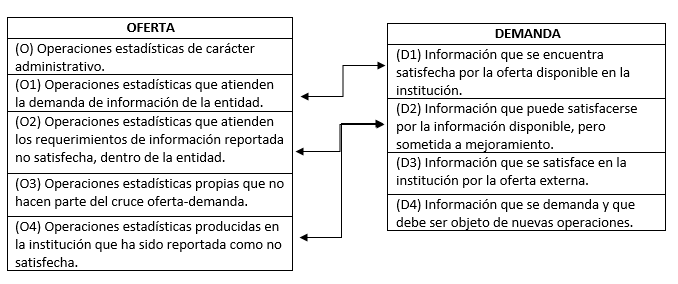
\includegraphics[width=0.8\linewidth]{Imagenes/ima1} 

}

\caption{Resultados del cruce de oferta-demanda}\label{fig:unnamed-chunk-2}
\end{figure}

Fuente: \protect\hyperlink{ref-maldonado2009metodologia}{Maldonado} (\protect\hyperlink{ref-maldonado2009metodologia}{2009}).

\begin{enumerate}
\def\labelenumi{\alph{enumi}.}
\setcounter{enumi}{2}
\tightlist
\item
  Analizar los requerimientos de información.
\end{enumerate}

\hypertarget{dignuxf3stico-clasificaciuxf3n-y-evaluaciuxf3n-de-la-oferta-y-la-demanda-de-operaciones-estaduxedsticas-e-indicadores}{%
\chapter{Dignóstico, clasificación y evaluación de la oferta y la demanda de operaciones estadísticas e indicadores}\label{dignuxf3stico-clasificaciuxf3n-y-evaluaciuxf3n-de-la-oferta-y-la-demanda-de-operaciones-estaduxedsticas-e-indicadores}}

La información necesaria para construir el inventario de información estadística se capturó en
cada una de las dependencias del nivel nacional de la UNAL. No obstante, los análisis de diagnóstico
son presentados a nivel de núcleos de información, aunque en su interior, las operaciones son
asociadas al responsable de su producción.

\hypertarget{diagnuxf3stico-de-la-oferta-de-operaciones-estaduxedsticas-1}{%
\section{Diagnóstico de la oferta de operaciones estadísticas}\label{diagnuxf3stico-de-la-oferta-de-operaciones-estaduxedsticas-1}}

Una vez aplicados los formularios de oferta y demanda de información estadística en todas las
dependencias, se contó con los insumos necesarios para realizar el diagnóstico de la información
estadística que produce la Universidad, que a su vez, es insumo fundamental para la formulación del
Plan. Dicho diagnóstico, incluyó tanto el análisis de oferta como el de demanda, con el fin de
establecer cuál era el estado real de la producción y en qué grado se satisfacen las necesidades de
información (internas y externas).

\hypertarget{anuxe1lisis-de-la-oferta-de-informaciuxf3n-1}{%
\subsection{Análisis de la oferta de información}\label{anuxe1lisis-de-la-oferta-de-informaciuxf3n-1}}

La oferta en este caso se entiende como la información producida y puesta a disposición de
posibles usuarios en un momento determinado. Para evaluar la oferta se tomó como primer
criterio de evaluación a modo de marco general, el carácter misional o estratégico de la
información producida por la UNAL. Lo anterior es claro en el sentido en que la producción de
estadísticas debe obedecer a las necesidades de información para la toma oportuna y acertada de
decisiones estratégicas de la Universidad, cabe aclararse, que no se desconoce la importancia de la
información estadística que permite medir y hacer seguimiento a la gestión de cada una de las
áreas vinculadas al proceso, solo que en el desarrollo del Plan se consideró la producción de
información estratégica.

Para la Universidad Nacional de Colombia se identificó una producción de 43 operaciones
estadísticas y 69 registros administrativos. A la totalidad de las operaciones documentadas se les
aplicó el proceso de revisión técnica y se sugirieron modificaciones para mejorar sus procesos de
producción.

\begin{table}

\caption{\label{tab:unnamed-chunk-3}Consolidado de Operaciones Estadísticas}
\centering
\begin{tabular}[t]{l|l|l}
\hline
Operación & Productor & Código\\
\hline
Consolidación de información de inscritos y admitidos a los programas curriculares de pregrado semestralmente por la Universidad Nacional de Colombia & Dirección Nacional de Admisiones & dna12:1\\
\hline
Consolidación de información de inscritos y admitidos a los programas curriculares de posgrado semestralmente por la universidad Nacional de Colombia & Dirección Nacional de Admisiones & dna12:3\\
\hline
Estadísticas de gestión anual del Sistema de Bienestar Universitario & Dirección Nacional de Bienestar Universitario & dnbu16:1\\
\hline
Medición de la Satisfacción del Usuario & Dirección Nacional de Bienestar Universitario & dnbu16:2\\
\hline
Identificación de potencialidades y vulnerabilidades al momento del ingreso para estudiantes de pregrado. & Dirección Nacional de Bienestar Universitario & dnbu16:3\\
\hline
Medición de Indicadores de Gestión & Dirección Nacional de Bienestar Universitario & dnbu16:4\\
\hline
Monitoreo de prensa & UNIMEDIOS & unimedios19:1\\
\hline
Seguimiento a las órdenes contractuales de prestación de servicios de personas naturales de la Universidad Nacional de Colombia & Gerencia Nacional Financiera y Administrativa & gnfa20:1\\
\hline
Informe Seguimiento a la información del proceso de Gestión de Bienes & Gerencia Nacional Financiera y Administrativa & gnfa20:2\\
\hline
Informe consolidado de Ejecución Presupuestal (Presupuesto) & Gerencia Nacional Financiera y Administrativa & gnfa20:3\\
\hline
Memoria Financiera (Gerencia Nacional Financiera y Administrativa) & Gerencia Nacional Financiera y Administrativa & gnfa20:4\\
\hline
Indicadores del proceso de Adquisición de Bienes y Servicios & Gerencia Nacional Financiera y Administrativa & gnfa20:5\\
\hline
Estadísticas de contratación & Gerencia Nacional Financiera y Administrativa & gnfa20:6\\
\hline
Estados Contables Consolidados UN & Gerencia Nacional Financiera y Administrativa & gnfa20:8\\
\hline
Seguimiento al sistema de peticiones de la Universidad Nacional & Vicerrectoría General & vrg21:1\\
\hline
Seguimiento a la rendición de cuentas & Oficina De Planeación Sede Bogotá & opb23:1\\
\hline
Consolidar las estadísticas de la Sede Bogotá & Oficina De Planeación Sede Bogotá & opb23:2\\
\hline
Seguimiento al Plan de Acción institucional & Oficina De Planeación Sede Bogotá & opb23:3\\
\hline
Libro de capacidades de Investigación de la Universidad Nacional de Colombia & Vicerrectoría de Investigación & vri25:1\\
\hline
Consolidación de la información estadística para los procesos de autoevaluación y evaluación continua & Dirección Nacional de Programas Curriculares de Posgrado & dnpr26:1\\
\hline
Consolidación de la movilidad estudiantil entrante y saliente & Oficina de Relaciones Exteriores & dre28:1\\
\hline
Convenios nacionales e internacionales & Oficina de Relaciones Exteriores & dre28:3\\
\hline
Indicadores opinión de apoyo a la autoevaluación de los programas de pregrado & Dirección Nacional de Programas Curriculares de Pregrado & dnpcp32:1\\
\hline
Indicadores estadísticos de apoyo a la autoevaluación de los programas de pregrado & Dirección Nacional de Programas Curriculares de Pregrado & dnpcp32:2\\
\hline
Consolidación de Estadísticas de Personal Académico y Administrativo & Dirección Nacional de personal académico y administrativo & dnpa33:1\\
\hline
Consolidación del Informe Docente & Dirección Nacional de personal académico y administrativo & dnpa33:2\\
\hline
Consolidación Programación anual Presupuesto Gastos de Nómina & Dirección Nacional de personal académico y administrativo & dnpa33:3\\
\hline
Consolidación del gasto mensualizado de nómina por sede (PAC - Plan anual mensualizado de caja) & Dirección Nacional de personal académico y administrativo & dnpa33:4\\
\hline
Informe anual costos de personal & Dirección Nacional de personal académico y administrativo & dnpa33:5\\
\hline
Construcción de la Revista de Estadísticas e indicadores de la Universidad Nacional de Colombia & Dirección Nacional de Planeación y Estadística & dnpe40:1\\
\hline
Seguimiento al Plan de Desarrollo de la Universidad Nacional de Colombia & Dirección Nacional de Planeación y Estadística & dnpe40:2\\
\hline
Distribución y seguimiento de los recursos de inversión & Dirección Nacional de Planeación y Estadística & dnpe40:3\\
\hline
Consolidación de Indicadores de Extensión de la Universidad Nacional de Colombia & Dirección Nacional de Extensión, Innovación y Propiedad Intelectual & dne41:2\\
\hline
Generador de indicadores & Dirección Nacional de Información Académica & sia61:1\\
\hline
Encuesta de satisfacción al usuario & Programa de egresados & pe78:1\\
\hline
Reporte mensual, Unidad del Servicio Público de Empleo & Programa de egresados & pe78:2\\
\hline
Reporte indicadores del Sistema Nacional de Bibliotecas & Oficina Nacional de Bibliotecas & sinab79:1\\
\hline
Consolidación de Procesos Judiciales y de conciliación de las Sedes & Dirección Jurídica Nacional & djn83:1\\
\hline
Consolidación de la información editorial de la Universidad Nacional de Colombia & Editorial UN & editorial84:1\\
\hline
Consolidado de indicadores ambientales de la Universidad Nacional & Sistema Gestión Ambiental & siga87:1\\
\hline
Consolidación de la medición de indicadores ambientales - GREENMETRIC & Sistema Gestión Ambiental & siga87:2\\
\hline
Consolidación de la información de encuestas para los procesos de autoevaluación y evaluación continua & Dirección Nacional de Programas Curriculares de Posgrado & dnpr26:2\\
\hline
Medición de la satisfacción del usuario & Vicerrectoría General & vrg21:2\\
\hline
\end{tabular}
\end{table}

\begin{table}

\caption{\label{tab:unnamed-chunk-4}Consolidado de Registros Administrativos RRAA}
\centering
\begin{tabular}[t]{l|l}
\hline
Productor & Nombre del registro administrativo RRAA\\
\hline
Dna & Reporte estándar del ISYSDNA para pregrado\\
\hline
Dnbu & Sistema de Información de Bienestar Universitario - SIBU\\
\hline
Dnbu & Encuesta de satisfacción\\
\hline
Dne & Consolidación de la información de HERMES\\
\hline
Dnpa & Planta Ocupada Personal Docente y Administrativo Sedes\\
\hline
Dnpa & Reporte Ranking QoS\\
\hline
Dnpa & Reporte Ranking THE\\
\hline
Dnpa & Reporte SNIES\\
\hline
Dnpa & Reporte Sistema de Autoevaluación Programas de Pregrado\\
\hline
Dnpa & Reporte Sistema de Autoevaluación Programas de Posgrado\\
\hline
Dnpa & Reporte conceptos de nómina por empleado para el Fondo Pensional\\
\hline
Dnpa & Información para Consejos Profesionales\\
\hline
Dnpa & Informe desfinanciación de la Educación en Colombia que lidera el SUE\\
\hline
Dnpa & Informe de rendición de cuentas a la Contraloría General de la República SIRECI\\
\hline
Dnpa & Informe ajustes presupuestales\\
\hline
Dnpa & Informe gastos de personal\\
\hline
Dnpa & Nómina intereses cesantías\\
\hline
Dnpa & Reporte informativo consolidación cesantías anuales\\
\hline
Dnpa & Informe gastos de nómina Vigilancia\\
\hline
Dnpa & Informe información exógena DIAN\\
\hline
Dnpa & Informe Índices de costos de la educación superior ICES\\
\hline
Dnpa & Reporte de productividad Académica\\
\hline
Dnpa & Reporte de reconocimiento de puntaje por títulos\\
\hline
Dnpa & Reporte de reconocimiento de puntaje por dirección de Tesis de Posgrado\\
\hline
Dnpa & Reporte Estadísticas concurso profesoral\\
\hline
Dnpa & Informe situaciones administrativas del Personal Docente\\
\hline
Dnpa & Informe de reconocimiento de tenencias de cargo\\
\hline
Dnpe & Consolidar y reportar información al Sistema de Rendición Electrónica de la Cuenta e Informes–SIRECI\\
\hline
Dnpe & Suministro de información al Sistema Nacional de Información de la Educación Superior SNIES\\
\hline
Dnpe & Información para el Sistema de Prevención y Análisis a la Deserción en las Instituciones de Educación Superior -SPADIES\\
\hline
Dnpe & Información para la elaboración del documento para la Calificadora de Riesgo\\
\hline
Dnpr & Registro de la información de los programas curriculares de posgrado en el Sistema Nacional de Información de Educación Superior (SNIES) a través del Sistema de Aseguramiento de la Calidad en la Educación Superior (SACES), sistemas adscritos al Ministerio de Educación Nacional (MEN)\\
\hline
Dre & Movilidad entrante, saliente, registro convenios\\
\hline
Editorial & Control ISBN\\
\hline
Gnfa & Reporte de Información general técnica, administrativa y jurídica sobre los activos inmobiliarios de la Universidad en el Sistema SIGA (Gestión de bienes)\\
\hline
Gnfa & Declaración y pago de Retención en la fuente (Tesorería)\\
\hline
Gnfa & Declaración y pago de retención de impuestos de industria y comercio de Bogotá (ICA)(Tesorería)\\
\hline
Gnfa & Informe Contribución 5\% de Obra Pública (Tesorería)\\
\hline
Gnfa & Informe Estampilla ProUniversidad Nacional de Colombia (Tesorería)\\
\hline
Gnfa & Informe Rendimientos Financieros Sistema General de Regalías (SGR) (Tesorería)\\
\hline
Gnfa & Informe de Inversiones Financieras - Artículo 58 Decreto 1525 de 2008 (Tesorería)\\
\hline
Gnfa & Reporte de información al SMSCE del módulo de cuentas del Sistema General de Regalías (SGR) – Ley 1530 del 17 de mayo de 2012 (Tesorería)\\
\hline
Gnfa & Reporte Informe CHIP (Presupuesto)\\
\hline
Gnfa & Reporte Informe CHIP REGALÍAS (Presupuesto)\\
\hline
Gnfa & Informe Balanza de pagos (Presupuesto)\\
\hline
Gnfa & Formato de rendición de cuentas SIRECI CGR:M-9. Gestión Contractual.\\
\hline
Gnfa & Formato de rendición de cuentas SIRECI CGR:M-1.Cuenta o informe anual consolidado (Formulario F2. Plan de Compras)\\
\hline
Gnfa & Formato de rendición de cuentas SIRECI CGR:M-11.1. Econom y finanzas (Formulario F50.7 Personal y costos-contratistas)\\
\hline
Gnfa & Muestra trimestral de Comercio Exterior de Servicios MTCES\\
\hline
Gnfa & Indice de Costos de la Educación Superior ICES\\
\hline
Gnfa & Informe de SARES Vigentes ( Adquisición de bienes y servicios)\\
\hline
Gnfa & Formato de Estampilla Pro Universidad Nacional de Colombia y demás Universidades estatales de Colombia ( Adquisición de Bienes y Servicios)\\
\hline
Gnfa & Formato de Registro Recaudo Contribución - FONSECON (Adquisición de Bienes y Servicios)\\
\hline
Gnfa & Declaración de ingresos y patrimonio - DIAN (Contable)\\
\hline
Gnfa & Reporte Boletín de Deudores Morosos del Estado (Contable)\\
\hline
Gnfa & Reporte para el Sistema Nacional de Información de la Educación Superior (SNIES). (Contable)\\
\hline
Gnfa & Información exógena de la Universidad. (Contable)\\
\hline
Pe & Registro de egresado\\
\hline
Sia & Sistema de Información Académica\\
\hline
Siga & Formato 8 del Reporte de la contraloría Controlaría General de la Nación\\
\hline
vrg & Reporte de quejas y reclamos\\
\hline
vrg & Seguimiento a los resultados de las Auditorías\\
\hline
vrg & Reporte MERCO\\
\hline
vrg & Sistema de Gestión Ambiental - GreenMetric\\
\hline
vri & Registro y seguimiento de proyectos de investigación o extensión con financiación externa\\
\hline
vri & Registro para ejecución y seguimiento de las convocatorias internas\\
\hline
vri & Registro de laboratorios y equipos\\
\hline
vri & Registro y administración de las colecciones\\
\hline
vri & Registro y administración de los grupos de investigación\\
\hline
\end{tabular}
\end{table}

\hypertarget{resultados-agregados-de-la-revisiuxf3n-de-operaciones-estaduxedsticas-ofertadas-por-las-dependencias-un}{%
\subsection{Resultados agregados de la revisión de operaciones estadísticas ofertadas por las dependencias UN}\label{resultados-agregados-de-la-revisiuxf3n-de-operaciones-estaduxedsticas-ofertadas-por-las-dependencias-un}}

Criterios definidos para el diagnostico de las operaciones estadísticas propias de las dependencias
del orden nacional de la Universidad Nacional de Colombia.

\hypertarget{documentaciuxf3n-tuxe9cnica-de-la-operaciuxf3n-estaduxedstica}{%
\subsubsection{Documentación técnica de la operación estadística}\label{documentaciuxf3n-tuxe9cnica-de-la-operaciuxf3n-estaduxedstica}}

Con este criterio se busca responder a la pregunta: ¿Qué tan documentada está la operación estadística en relación a los parámetros establecidos en los campos de la ficha técnica?

\hypertarget{completitud-ficha-tuxe9cnica}{%
\paragraph{Completitud Ficha técnica}\label{completitud-ficha-tuxe9cnica}}

Verificación del nivel de diligenciamiento de los campos de la ficha técnica de la operación estadística documentada por el área o dependencia productora.

\begin{figure}
\centering
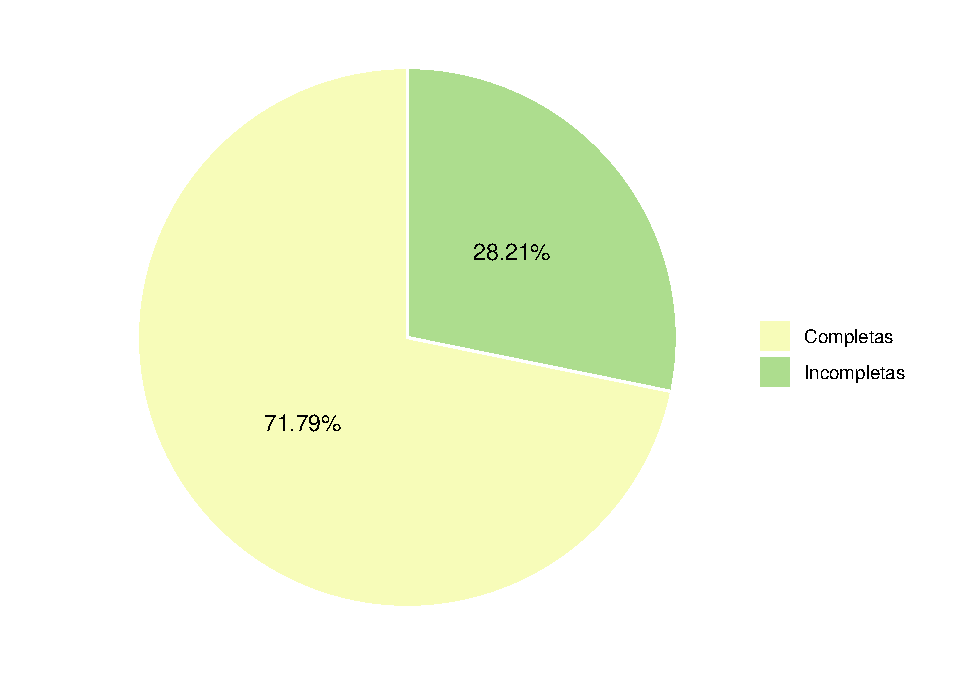
\includegraphics{Plan-Estadistico_files/figure-latex/unnamed-chunk-5-1.pdf}
\caption{\label{fig:unnamed-chunk-5}Resultados de Completitud de las Operaciones Estadisticas Ofertadas}
\end{figure}

\hypertarget{validez-de-contenido}{%
\paragraph{Validez de contenido}\label{validez-de-contenido}}

Se hace la verificación de que el contenido en los campos de la ficha técnica guarde correspondencia con lo indagado en cada uno de los ítems.

\begin{figure}
\centering
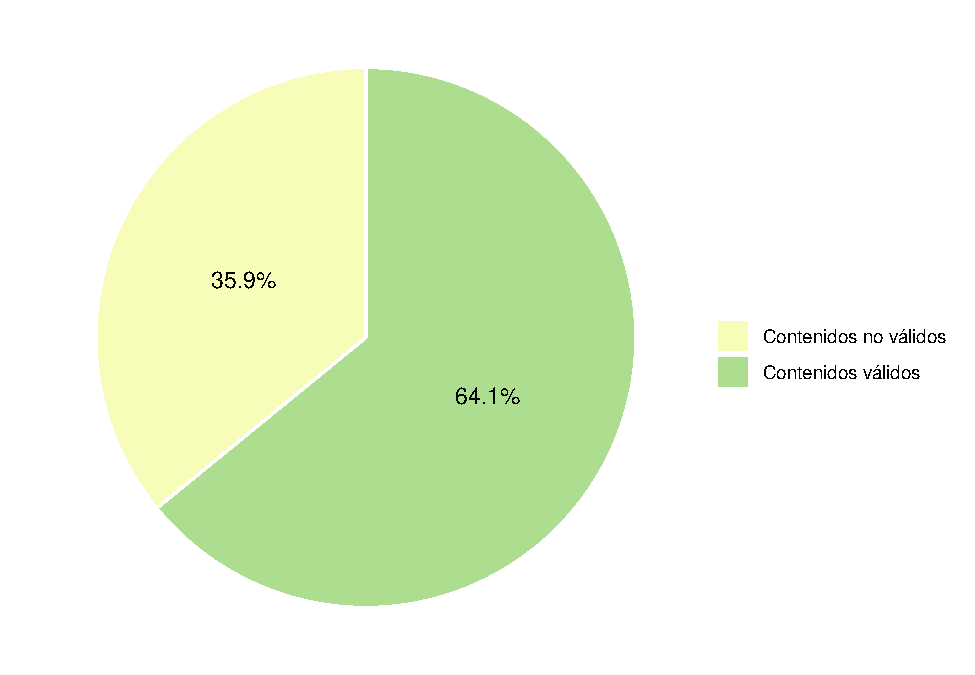
\includegraphics{Plan-Estadistico_files/figure-latex/unnamed-chunk-6-1.pdf}
\caption{\label{fig:unnamed-chunk-6}Resultados de Validez de contenido de OE}
\end{figure}

\hypertarget{calidad-del-proceso-estaduxedstico}{%
\subsubsection{Calidad del Proceso estadístico}\label{calidad-del-proceso-estaduxedstico}}

\hypertarget{accesibilidad}{%
\paragraph{Accesibilidad}\label{accesibilidad}}

Facilidad con que la información estadística puede ser ubicada y obtenida por los usuarios. Contempla la forma en que ésta se provee, los medios de difusión, así como la disponibilidad de las fichas técnicas y los servicios de apoyo para su consulta. Se verifica si los
resultados de la operación estadística, se divulgan por medios de mayor difusión como página web o sistema de información de manera que los distintos usuarios pueden acceder fácilmente a éstos. De los resultados de estos criterios se asigna una calificación para la operación entre el rango de 0-4.

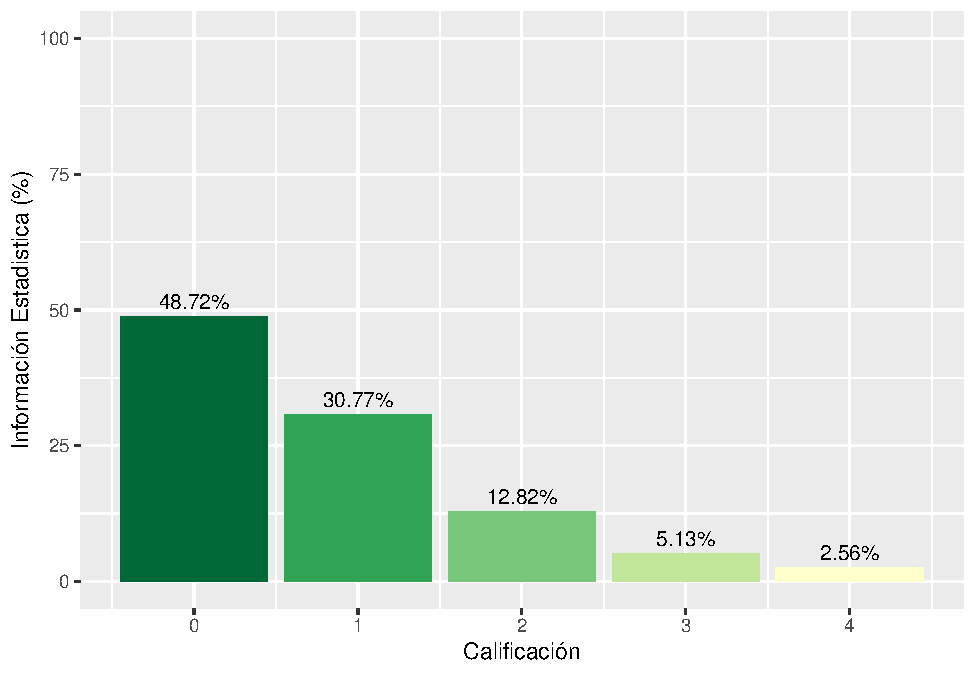
\includegraphics{Plan-Estadistico_files/figure-latex/unnamed-chunk-8-1.pdf}

\hypertarget{coherencia}{%
\paragraph{Coherencia}\label{coherencia}}

Se refiere al grado en que están lógicamente conectados los conceptos utilizados, las metodologías aplicadas y los resultados producidos por la operación. Verifica la consistencia lógica entre todos los elementos que hacen parte de la ficha e identifica las posibles contradicciones o ambigüedades que puedan existir entre los campos diligenciados.

\begin{figure}
\centering
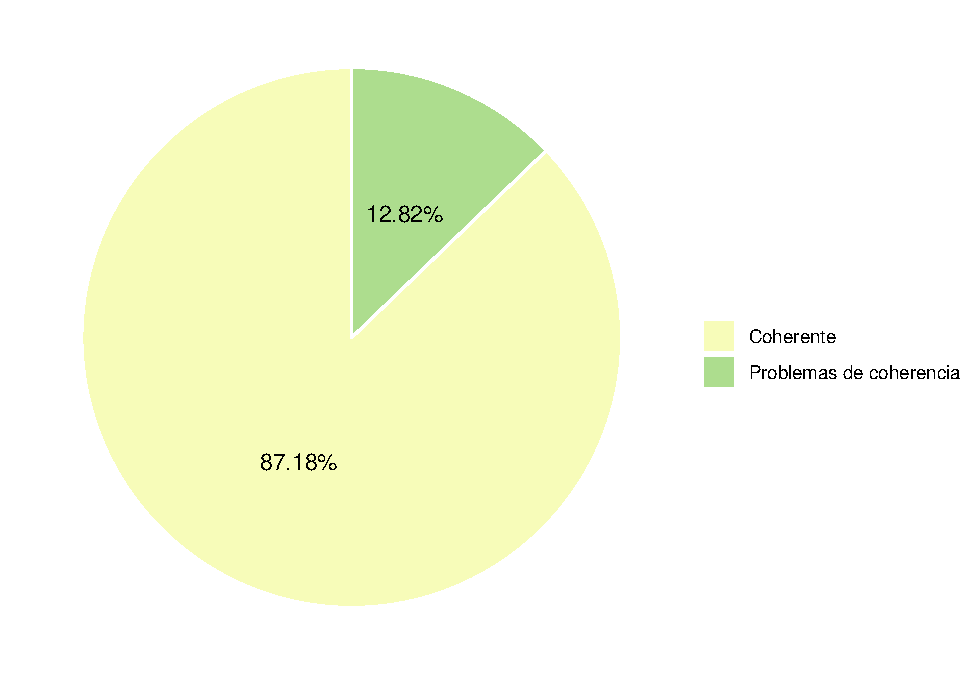
\includegraphics{Plan-Estadistico_files/figure-latex/unnamed-chunk-9-1.pdf}
\caption{\label{fig:unnamed-chunk-9}Resultados de Coherencia de OE}
\end{figure}

\hypertarget{continuidad}{%
\paragraph{Continuidad}\label{continuidad}}

Hace referencia a la garantía de la producción permanente de la operación
estadística, basada en la adecuación de los recursos así como en el soporte normativo.

\begin{figure}
\centering
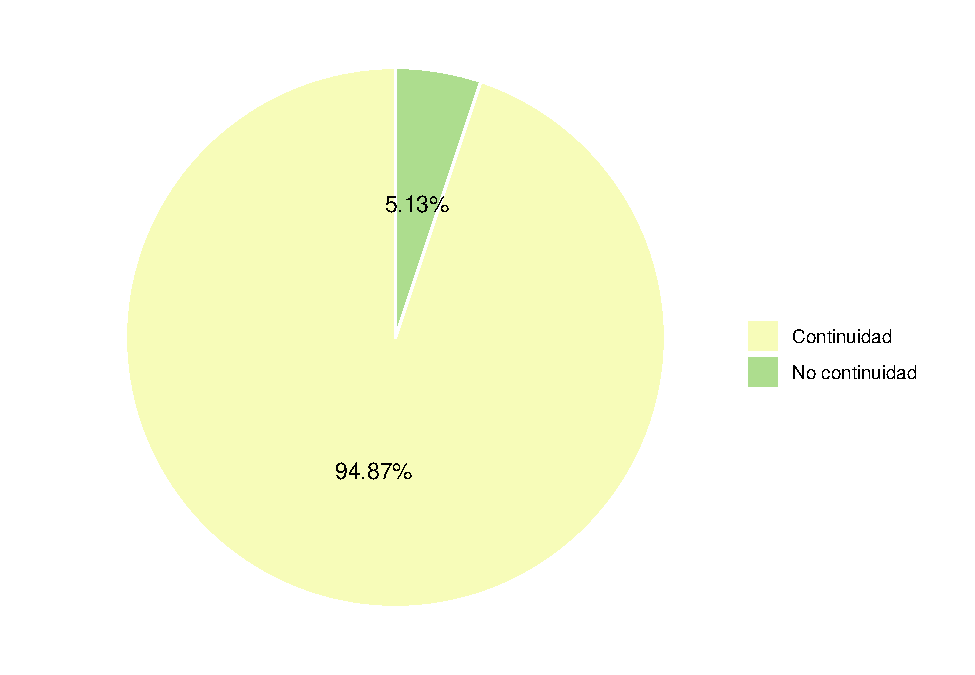
\includegraphics{Plan-Estadistico_files/figure-latex/unnamed-chunk-10-1.pdf}
\caption{\label{fig:unnamed-chunk-10}Resultados de Continuidad de OE}
\end{figure}

\hypertarget{exactitud}{%
\paragraph{Exactitud}\label{exactitud}}

Grado en que los resultados de la operación estadística se aproximan y describen correctamente las cantidades o características que se desean medir.

\begin{figure}
\centering
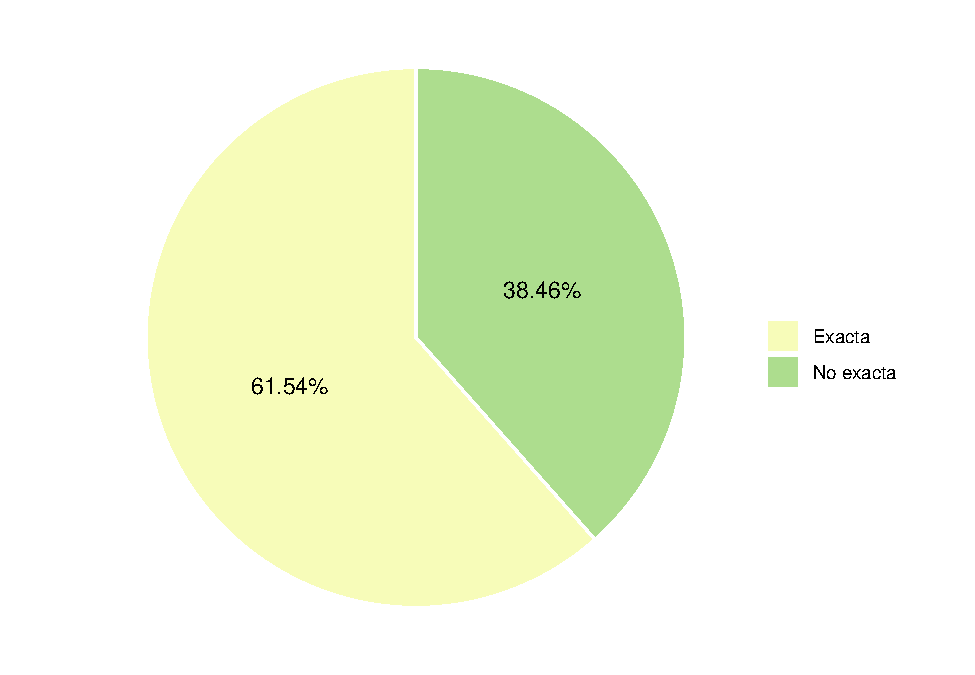
\includegraphics{Plan-Estadistico_files/figure-latex/unnamed-chunk-11-1.pdf}
\caption{\label{fig:unnamed-chunk-11}Resultados de Exactitud de OE}
\end{figure}

\hypertarget{interpretabilidad}{%
\paragraph{Interpretabilidad}\label{interpretabilidad}}

Facilidad con la que el usuario puede entender, utilizar y analizar los datos;
teniendo en cuenta el alcance de los mismos, en otros términos, se trata de indagar si en la ficha
se identifica claramente el ¿qué?, ¿para qué? y el ¿cómo? se adelanta la operación estadística.

\begin{figure}
\centering
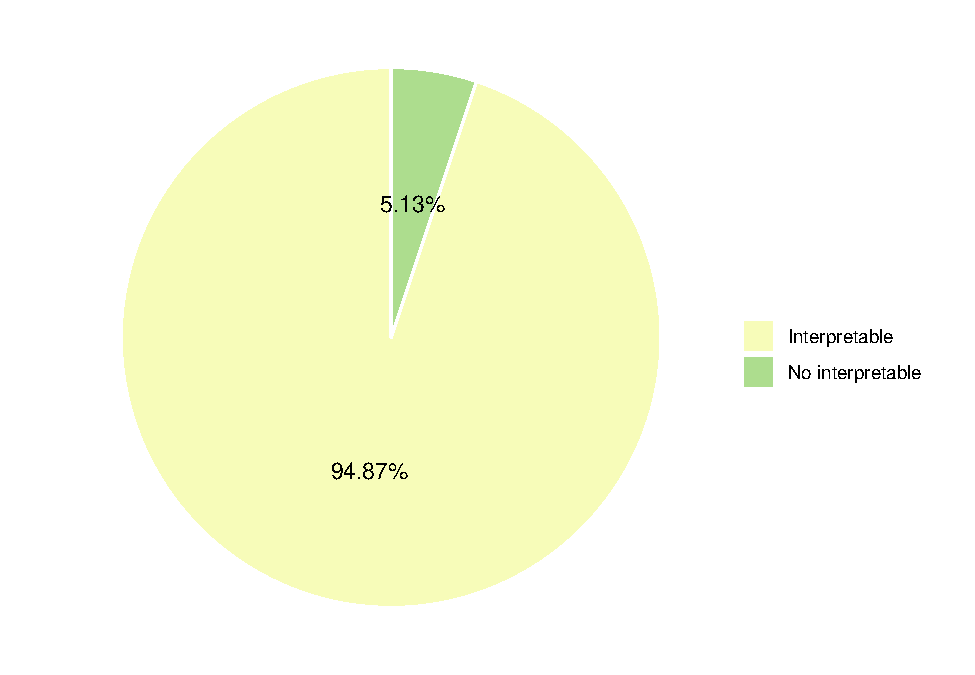
\includegraphics{Plan-Estadistico_files/figure-latex/unnamed-chunk-12-1.pdf}
\caption{\label{fig:unnamed-chunk-12}Resultados de Interpretabilidad de OE}
\end{figure}

\hypertarget{oportunidad}{%
\paragraph{Oportunidad}\label{oportunidad}}

Se refiere al tiempo que transcurre entre la ocurrencia del fenómeno de estudio y la publicación de la información estadística, de tal manera que sea útil para la toma de decisiones. Se verifica si las estadísticas producidas se difunden de manera oportuna, esto es, si la periodicidad de producción del último dato y difusión son coherentes y no distan en más de un periodo una de la otra.

\begin{figure}
\centering
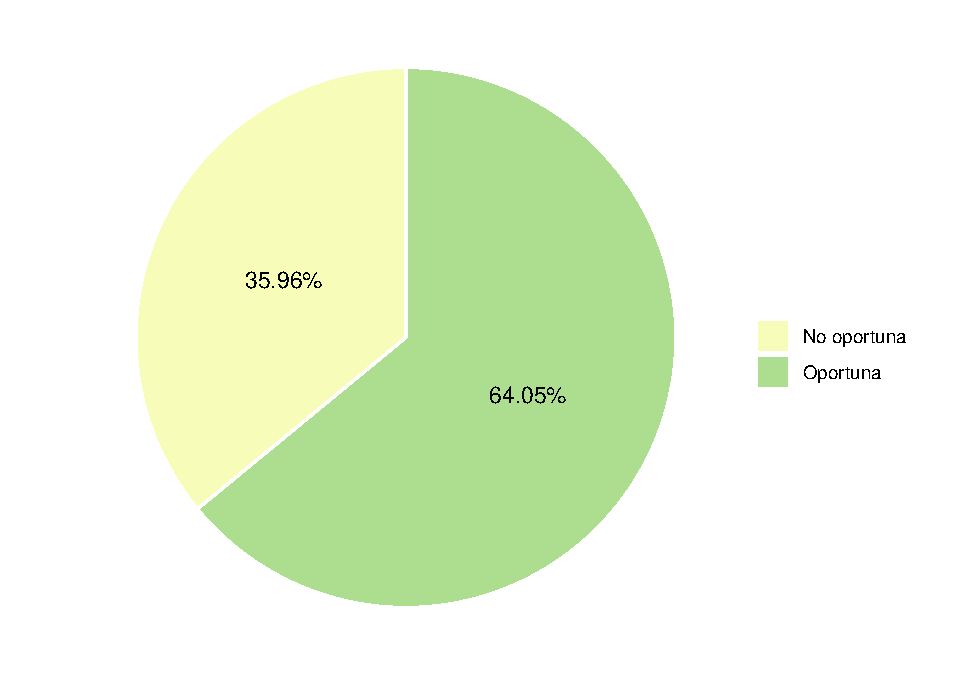
\includegraphics{Plan-Estadistico_files/figure-latex/unnamed-chunk-13-1.pdf}
\caption{\label{fig:unnamed-chunk-13}Resultados de Oportunidad de OE}
\end{figure}

\hypertarget{relevancia}{%
\paragraph{Relevancia}\label{relevancia}}

Se refiere al grado en que las estadísticas satisfacen necesidades de información de
usuarios internos o externos.

\begin{figure}
\centering
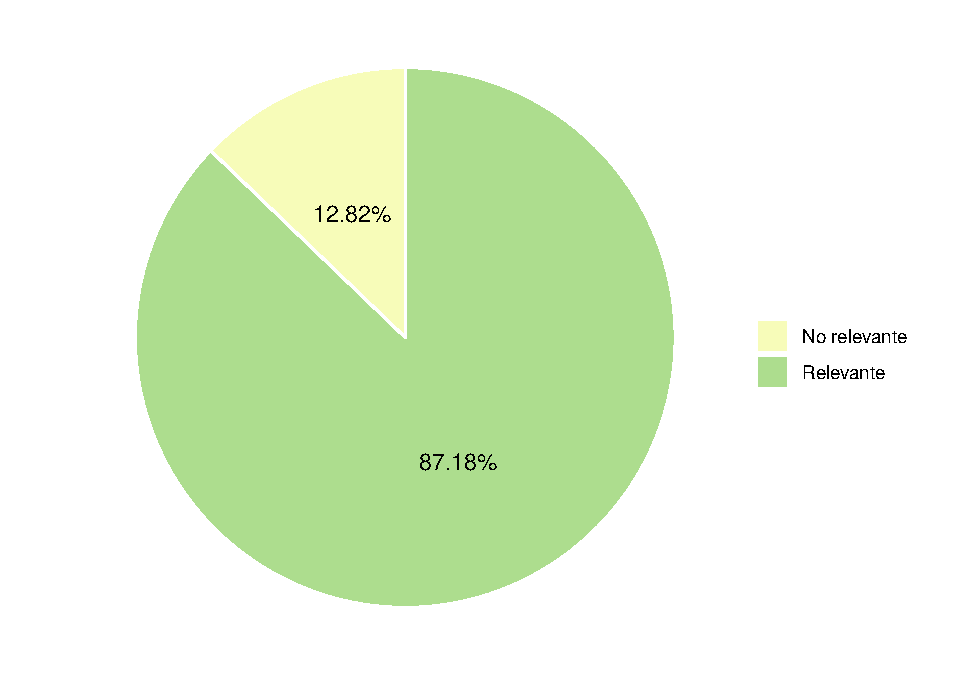
\includegraphics{Plan-Estadistico_files/figure-latex/unnamed-chunk-14-1.pdf}
\caption{\label{fig:unnamed-chunk-14}Resultados de Relevancia de OE}
\end{figure}

\hypertarget{transparencia}{%
\paragraph{Transparencia}\label{transparencia}}

Condición bajo la cual el productor de estadísticas pone a disposición de los
usuarios los metadatos que permiten conocer el desarrollo de la operación estadística.

\begin{figure}
\centering
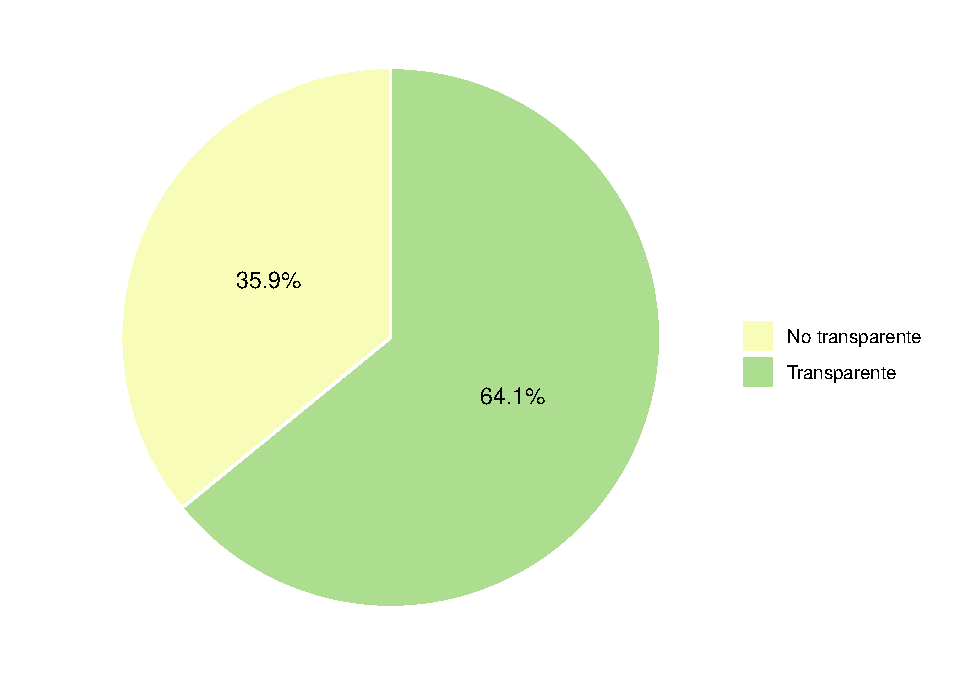
\includegraphics{Plan-Estadistico_files/figure-latex/unnamed-chunk-15-1.pdf}
\caption{\label{fig:unnamed-chunk-15}Resultados de Transparencia de OE}
\end{figure}

\hypertarget{anuxe1lisis-descriptivo-de-la-informaciuxf3n-demandada}{%
\subsection{Análisis descriptivo de la información demandada}\label{anuxe1lisis-descriptivo-de-la-informaciuxf3n-demandada}}

La demanda de información es entendida como el conjunto de requerimientos de información de
las diferentes dependencias o equipos de trabajo, necesarios para cumplir con su misionalidad,
planes de acción y/o atender los requerimientos internos o externos.

Se registró un total de 47 demandadas de información, en 36 de ellas se cuenta con el
requerimiento que es suministrado directamente por parte de sus productores, la mayoría son
producidas por dependencias o áreas internas, en 8 casos los productores son externos, las entidades son el ICFES, bases bibliográficas WOS -- SCOPUS, Colciencias, Ministerio de Educación,
Superintendencia de Inductria y Comercio - SIC y la Organización Mundial de la Propiedad Intelectual - OMPI.

En el caso de la información con la que no se cuenta, una de estas demandas es producida por el
Ministerio de Educación, el Observatorio de la Educación Superior y Observatorio Laboral de la Educación - OLE. En las otras 10 demandas
se identificaron áreas o dependencias internas como sus productores.

Para 39 demandas, la información se pude obtener de forma gratuita, 3 la obtienen por convenio y
otras 3 por solicitud; solo en un caso, la información es comprada. En la demanda restante se
registró para esta pregunta un valor no válido como respuesta.

\begin{figure}
\centering
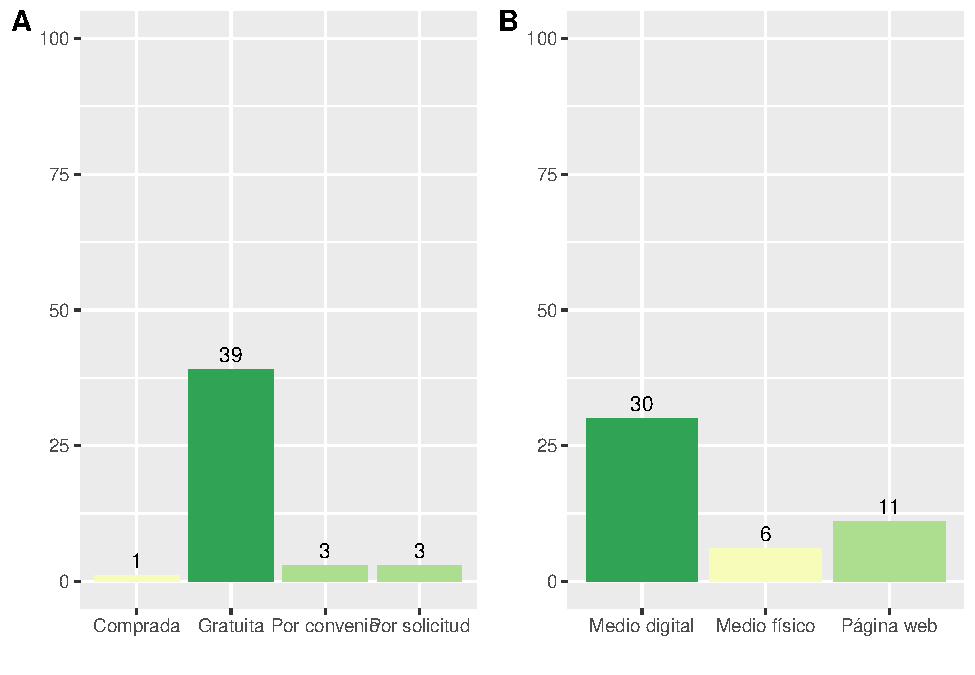
\includegraphics{Plan-Estadistico_files/figure-latex/unnamed-chunk-20-1.pdf}
\caption{\label{fig:unnamed-chunk-20}Forma de obtención de la información vs.~Medio de obtención de la información}
\end{figure}

El nivel de satisfacción de necesidades con información obtenida no es muy alto, apenas en el 43\% que, corresponde a 20 demandas, la satisfacción es total. En el 36\%, que corresponde a 17 demandas, la satisfacción es parcial y mínima para el 13\%. En los casos restantes no se tiene respuesta a esta pregunta.

\begin{figure}
\centering
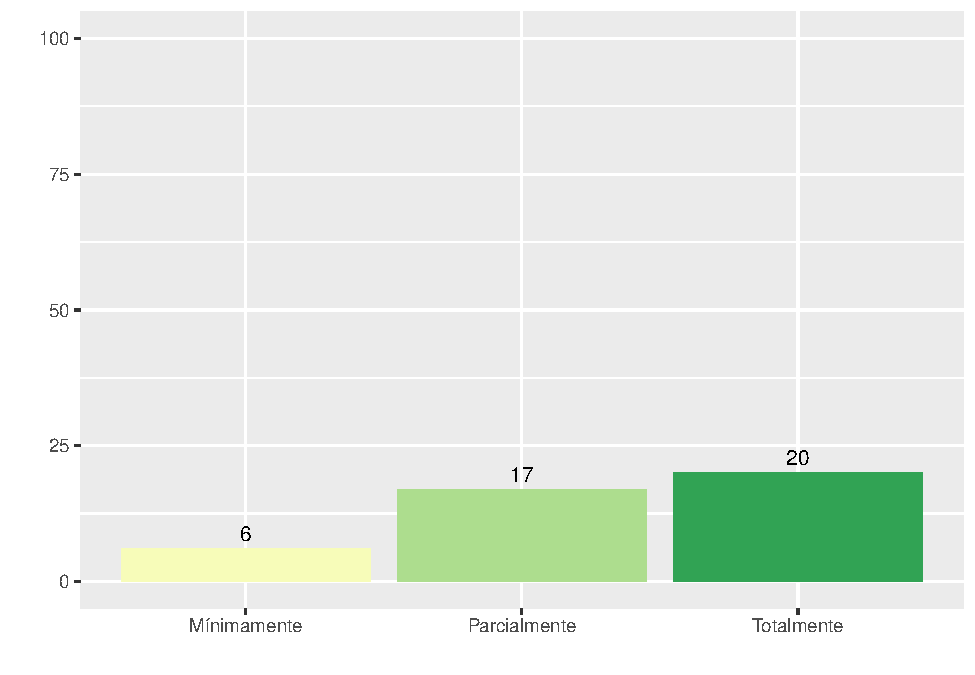
\includegraphics{Plan-Estadistico_files/figure-latex/unnamed-chunk-22-1.pdf}
\caption{\label{fig:unnamed-chunk-22}Nivel de Satisfacción de Necesidades}
\end{figure}

En 11 de las demandas que corresponden al 23\% nunca se han presentado inconsistencias, en el
49\% algunas veces, y en el 13\% siempre se presentan inconsistencias. En los casos restantes no se
tiene respuesta a esta pregunta.

\begin{figure}
\centering
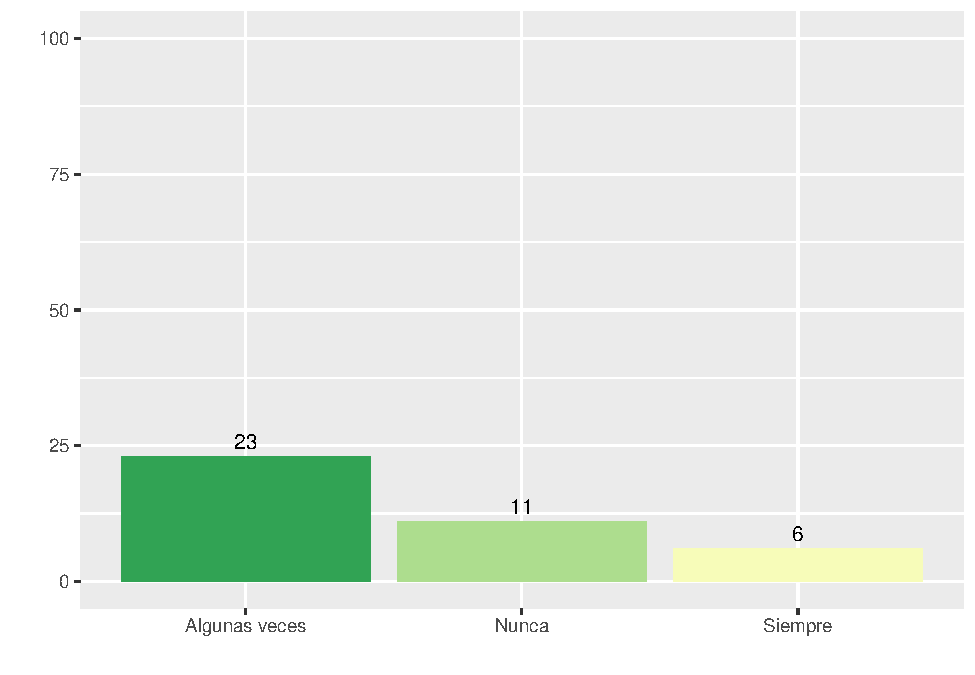
\includegraphics{Plan-Estadistico_files/figure-latex/unnamed-chunk-24-1.pdf}
\caption{\label{fig:unnamed-chunk-24}Frecuencia de inconsistencias en la información entregada}
\end{figure}

El principal uso de la información demandada es la producción de estadísticas. En segundo lugar, el diseño, la formulación y el seguimiento a planes, programas o proyectos y, en tercer lugar, el análisis de contexto.

\begin{figure}
\centering
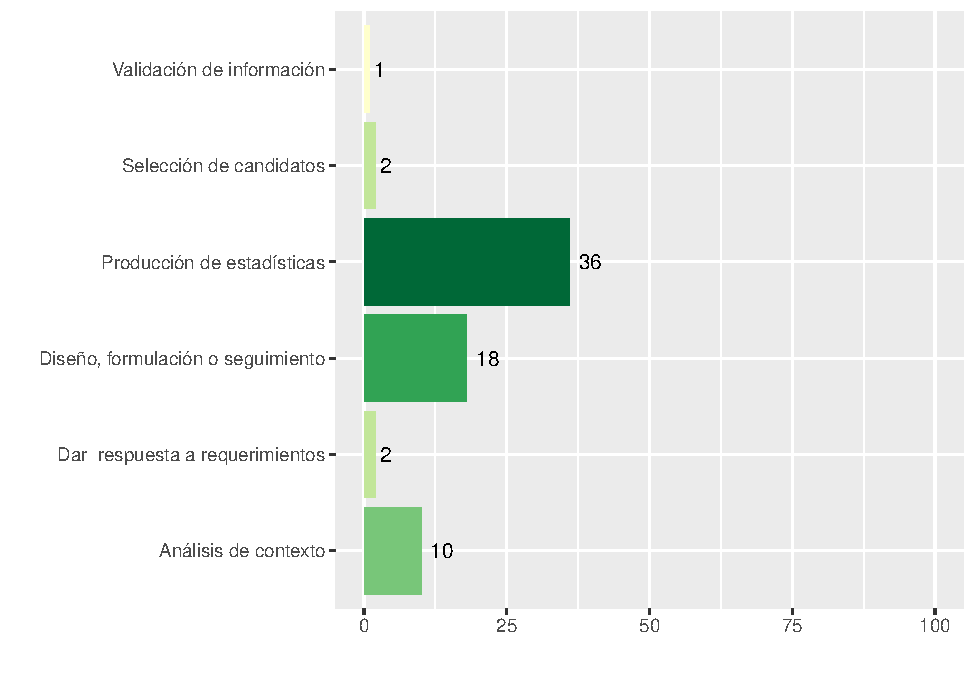
\includegraphics{Plan-Estadistico_files/figure-latex/unnamed-chunk-26-1.pdf}
\caption{\label{fig:unnamed-chunk-26}Usos de la información demandada}
\end{figure}

\hypertarget{registros-administrativos-rraa}{%
\subsection{Registros administrativos (RRAA)}\label{registros-administrativos-rraa}}

Como resultados de la indagación de información estadística usada o producida por las diferentes
áreas o dependencias que conforman el nivel central de la Universidad Nacional, se identificó que
buena parte de la información estadística producida usa como fuente primaria de datos la
información consolidada mediante registros administrativos,\footnote{Un registro administrativo se define como todo registro resultante de necesidades fiscales, tributarias u otras, creado con la finalidad de viabilizar la administración de los programas de gobierno o para fiscalizar el
  cumplimento de obligaciones legales de la sociedad. Registros administrativos, calidad de los datos y
  credibilidad pública. Véase \protect\hyperlink{ref-echegoyen2004registros}{Echegoyen} (\protect\hyperlink{ref-echegoyen2004registros}{2004})} en ese sentido, cada dependencia
adelantó en un formato estándar la documentación de las características técnicas de los registros
que están bajo su responsabilidad, en total se identificaron y diligenciaron sesenta y nueve
registros administrativos los cuales, para su consulta y potencial uso estadístico, fueron
relacionados en una base de datos.

A los registros reportados por las dependencias se les aplicó un proceso de revisión en tres
criterios específicos: completitud, validez de contenido y coherencia. Los resultados generales del
proceso se resumen en los siguientes gráficos.

\begin{figure}
\centering
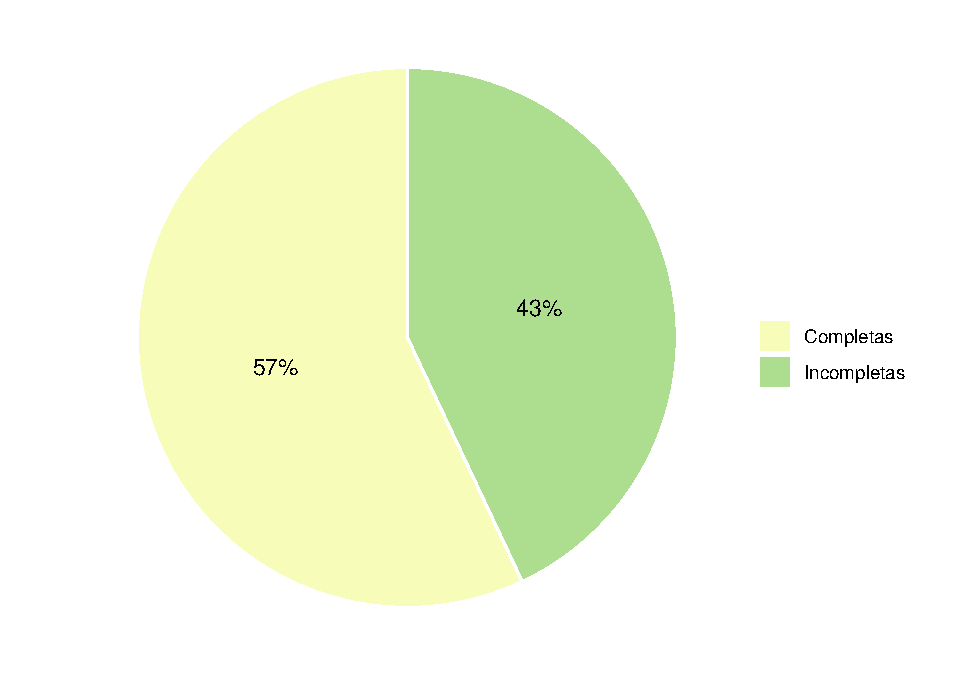
\includegraphics{Plan-Estadistico_files/figure-latex/unnamed-chunk-27-1.pdf}
\caption{\label{fig:unnamed-chunk-27}Completitud de las fichas de RRAA}
\end{figure}

Dentro de las principales razones de no completitud de las fichas, se destaca la no especificación
de si la información consolidada mediante el registro administrativo es insumo para la medición de
indicadores o si son parte de operaciones estadísticas. También se identificaron problemas en la
definición de población objetivo y las variables que se incluyen en el registro.

\begin{figure}
\centering
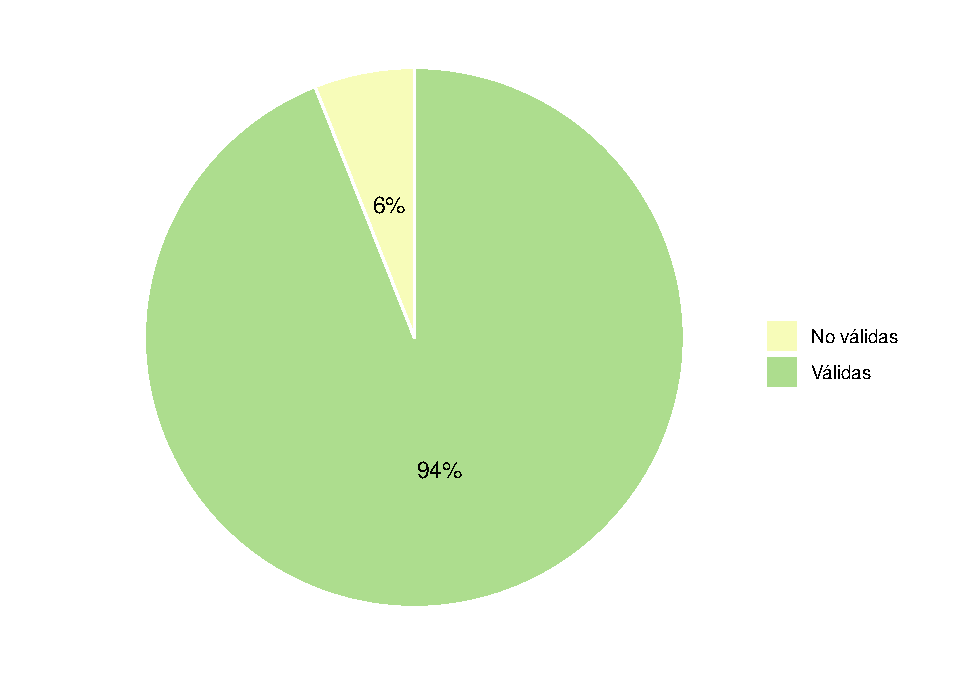
\includegraphics{Plan-Estadistico_files/figure-latex/unnamed-chunk-28-1.pdf}
\caption{\label{fig:unnamed-chunk-28}Validez de contenido de las fichas de RRAA}
\end{figure}

Los problemas de validez de contenido se refieren básicamente a la definición de los objetivos y de
las unidades de observación correspondiente al registro administrativo.

\begin{figure}
\centering
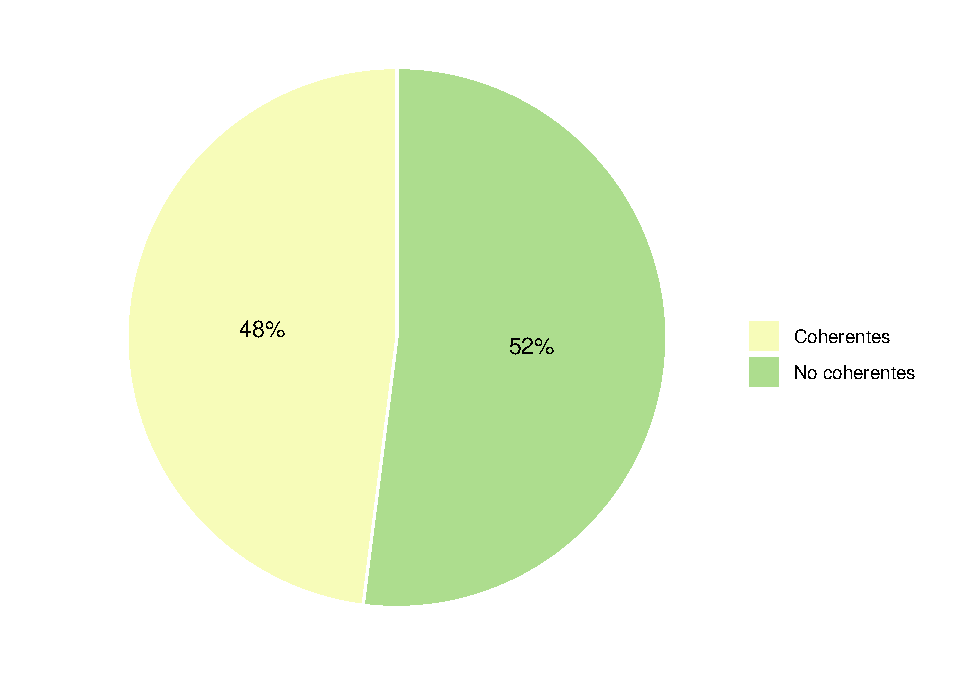
\includegraphics{Plan-Estadistico_files/figure-latex/unnamed-chunk-29-1.pdf}
\caption{\label{fig:unnamed-chunk-29}Coherencia de las fichas de RRAA}
\end{figure}

Dentro de los problemas de incoherencias más frecuentes se encontró la no correspondencia entre
la descripción del registro administrativo y la unidad de observación relacionada.

\hypertarget{cruce-oferta-demanda}{%
\subsection{Cruce oferta demanda}\label{cruce-oferta-demanda}}

Para la Universidad Nacional de Colombia se identificó una producción de 43 operaciones
estadísticas y 69 registros administrativos, por otro lado, se reportó una demanda (satisfecha e
insatisfecha) de 53 requerimientos de información estadística. El ejercicio de cruce de oferta
demanda, consiste en establecer flujos de información y en identificar qué operaciones
estadísticas pueden ser fuente para suplir estas necesidades o demandas de información.

\textbf{Flujos de información}

De los 53 requerimientos de información, 43 están siendo satisfechos, total o parcialmente por las
operaciones estadísticas reportadas en la oferta, o por alguna otra fuente de información. A continuación, se presenta los flujos de información indicando las áreas demandantes con los
códigos de los requerimientos de información, y frente a ellos, el código de la operación
estadística que satisface este requerimiento junto a su área productora, o el nombre del registro
administrativo, esto en el caso de ser producidos por la Entidad y haber sido documentados
dentro del inventario del Plan Estadístico. En caso contrario se indica el nombre de las entidades
productoras o de las otras fuentes que estén siendo utilizadas para tomar la información. En el
caso en el que los requerimientos no estén siendo satisfechos, el diagrama muestra el comentario:
``No cuenta con la información.''

\begin{figure}

{\centering 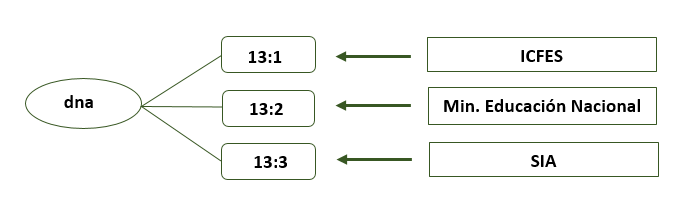
\includegraphics[width=0.75\linewidth]{Imagenes/ima2} 

}

\caption{DNA}\label{fig:unnamed-chunk-30}
\end{figure}

La DNA presentó tres requerimientos, y cuenta con esta información, considera la información
suministrada satisface completamente sus necesidades.

\begin{figure}

{\centering 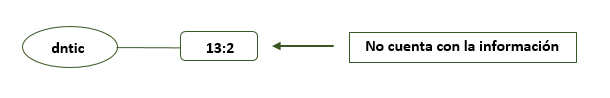
\includegraphics[width=0.75\linewidth]{Imagenes/ima3} 

}

\caption{DNTIC}\label{fig:unnamed-chunk-31}
\end{figure}

La DNTIC presentó el requerimiento 17:1 \emph{``Información del inventario semestral de activos tecnológicos de Hardware y software de la Universidad Nacional''} con el cual no cuenta, de
acuerdo a la información documentadas, se considera que la operación 25:1 \emph{``Indicadores del proceso de Adquisición de Bienes y Servicios''} de la GNFA, podría ser una fuente de información y,
otra posible fuente, sería el registro administrativo 42:1 \emph{``Reporte de Información general técnica, administrativa y jurídica sobre los activos inmobiliarios de la Universidad en el Sistema SIGA (Gestión de bienes)''} también de esta área.

\begin{figure}

{\centering 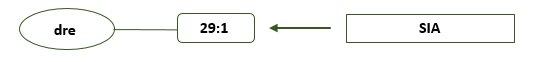
\includegraphics[width=0.75\linewidth]{Imagenes/ima4} 

}

\caption{DNTIC}\label{fig:unnamed-chunk-32}
\end{figure}

Para la DRE, la información suministrada por el SIA para su requerimiento 29:1 \emph{``Registros completos y oportunos de las movilidades efectivas entrantes y salientes''} satisface parcialmente
sus necesidades de información, esto debido a que las sedes, a quienes se les solicita la
información en muchas ocasiones no tienen esta información consolidada.

\begin{figure}

{\centering 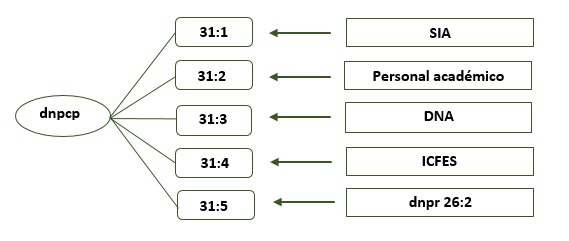
\includegraphics[width=0.75\linewidth]{Imagenes/ima5} 

}

\caption{DNPCP}\label{fig:unnamed-chunk-33}
\end{figure}

Para la DNPCP, la información suministrada para sus requerimientos: \emph{``Registros académicos periódicos -- SIA (31:1)''} y \emph{``Registros académicos periódicos -- DNA''} (31:3), satisfacen
parcialmente sus necesidades de información. El motivo es que cada usuario no tiene un
identificador entre las diferentes bases de datos, aunque estas son de la misma Universidad. Para
sus otros tres requerimientos la satisfacción con la información suministrada es completa.

\begin{figure}

{\centering 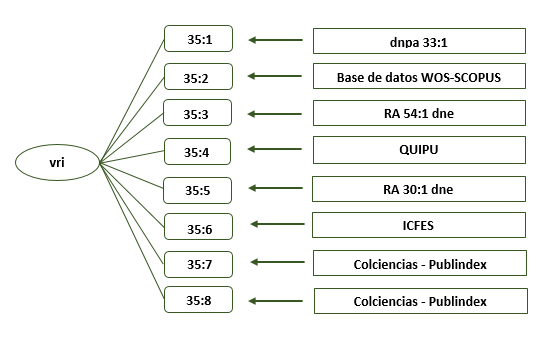
\includegraphics[width=0.75\linewidth]{Imagenes/ima6} 

}

\caption{VRI}\label{fig:unnamed-chunk-34}
\end{figure}

La VRI presenta ocho requerimientos de información, seis de ellos tienen un nivel parcial de
satisfacción con la información que les es suministrada. A continuación, se describen estos requerimientos, así como sus motivos de insatisfacción.

\begin{enumerate}
\def\labelenumi{\arabic{enumi}.}
\item
  Base de datos de producción académica, personal docente, comisiones de estudio (35:1),
  motivo: La producción académica y el personal docente requiere ser clasificado por áreas
  de conocimiento y agendas de conocimiento, categorías que desde el registro
  administrativo no se obtienen.
\item
  Base de datos de producción académica WOS y SCOPUS (35:2), motivo: El registro de la
  información no es homogéneo, requiere depuración y normalización de datos.
\item
  Información de movilidad y avales (35:4), motivo: El registro administrativo no se suministra
  oportunamente por parte de las facultades.
\item
  Base de datos de proyectos de investigación (35:5), motivo: Se requiere normalizar y
  clasificar datos.
\item
  Información de convenios (35:6), motivo: Se requiere mayor información de cada
  convenio: Año de suscripción, fecha de inicio, fecha de terminación, país, nombre de la institución, objeto del convenio, sede que coordina, facultad que coordina, profesor que coordina, área de conocimiento y tipo de convenio.
\item
  Base de datos de grupos de investigación e investigadores (35:8), motivo: La información
  procede de una base de datos Oracle de la cual se deben extraer los datos, han codificado
  variables y no se tiene acceso a qué corresponden los códigos.
\end{enumerate}

\begin{figure}

{\centering 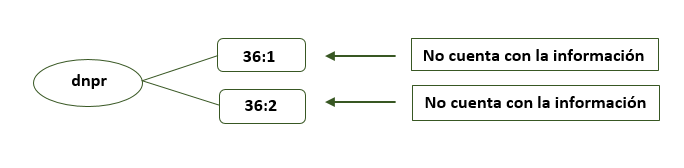
\includegraphics[width=0.75\linewidth]{Imagenes/ima7} 

}

\caption{DNPR}\label{fig:unnamed-chunk-35}
\end{figure}

La dependencia DNPR tiene dos requerimientos de información \emph{``Valoración de la calidad de losproductos académicos -artículos científicos- producidos por la comunidad Académica de la Universidad (factor de impacto, cuartil, etc.)''} y \emph{``Citas y co-citaciones de artículos científicos producidos por la comunidad Académica de la Universidad''} esta demanda está completamente
insatisfecha, y no fue posible identificar entre las operaciones y registros documentados en el Plan
Estadístico información que pudiera satisfacerla, por ello se hace necesario identificar qué área
podría y tendría la responsabilidad de producirla.

\begin{figure}

{\centering 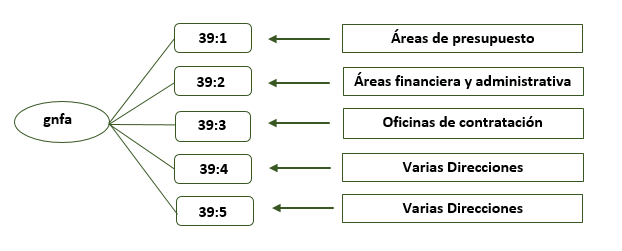
\includegraphics[width=0.75\linewidth]{Imagenes/ima8} 

}

\caption{GNFA}\label{fig:unnamed-chunk-36}
\end{figure}

En cuatro de los cinco requerimientos reportados por la GNFA, la satisfacción con la información
que les es suministrada por otras áreas o Entidades es completa; para el requerimiento 39:5
\emph{``Implementación del Sistema de Costos de la Universidad Nacional de Colombia''} la satisfacción es
parcial, la razón es que la información remitida por las dependencias requieren un procesamiento
para poder presentar información desagregada por programa curricular.

\begin{figure}

{\centering 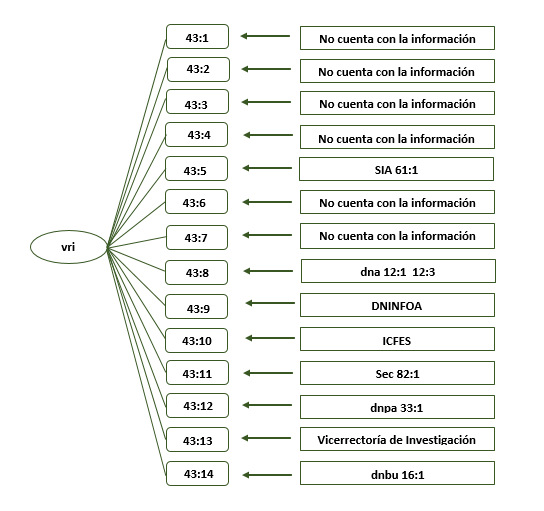
\includegraphics[width=0.6\linewidth]{Imagenes/ima9} 

}

\caption{DNPE}\label{fig:unnamed-chunk-37}
\end{figure}

La DNPE reporta 14 requerimientos de información, de ellos, dos reportaron tener una
satisfacción parcial con la información recibida, el 43:12 \emph{``Talento humano (Docentes y administrativos)''}, el motivo es que no cuentan con el nivel de formación de los empleados
administrativos. Y el 43:15 \emph{``Bienestar Universitario''}, pero no se reportó el motivo.

Los requerimientos 43:1 \emph{``Movilidad entrante de docentes y administrativos''}, 43:2 \emph{``Indicadores de infraestructura física''}, 43:7 \emph{``Egresados de la Universidad Nacional de Colombia''}, son demandas
insatisfechas de información y no se identificaron operación o registros que pudieran generarla.
Dos posibles fuentes para la producción del requerimiento 43:3, \emph{``Información ambiental''}, son las
operaciones 87:1 y 87:2, \emph{``Consolidado de indicadores ambientales de la Universidad Nacional''} y
\emph{``GREENMETRIC''} del SIGA, ó el registro administrativo 51:4 \emph{``Sistema de Gestión Ambiental - GREENMETRIC''} de la VRG.

El requerimiento 43:4 \emph{``Información de infraestructura tecnológica''} puede tener como fuente el
registro administrativo 34:3 \emph{``Registro de laboratorios y equipos''} de la VRI.

El requerimiento 43:6 puede tener tres posibles fuentes de información, las operaciones 33:1
\emph{``Consolidación de Estadísticas de Personal Académico y Administrativo''}, 12:1 \emph{``Consolidación de información de inscritos y admitidos a los programas curriculares de pregrado semestralmente por la universidad Nacional de Colombia''} y 12:3 \emph{``Consolidación de información de inscritos y admitidos a los programas curriculares de posgrado semestralmente por la universidad Nacional de Colombia''}.

\begin{figure}

{\centering 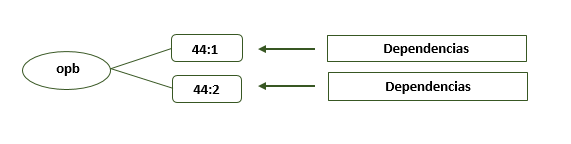
\includegraphics[width=0.75\linewidth]{Imagenes/ima10} 

}

\caption{OPB}\label{fig:unnamed-chunk-38}
\end{figure}

Los requerimientos de información de la OPB están completamente satisfechos.

\begin{figure}

{\centering 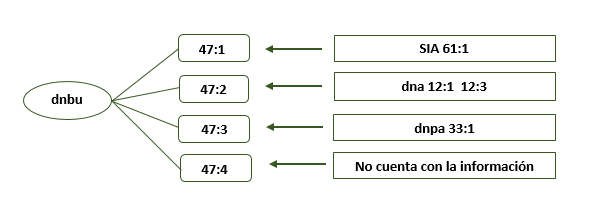
\includegraphics[width=0.75\linewidth]{Imagenes/ima11} 

}

\caption{DNBU}\label{fig:unnamed-chunk-39}
\end{figure}

Los requerimientos de la DNBU 47:1, 47:2 y 47:3 están completamente satisfechos para el área, en
cuanto al requerimiento 47:4'' Información de estudiantes y servidores públicos docentes y
administrativos insatisfecha'', ellos mencionan que no cuentan con toda la información que
necesitan, no fue posible identificar una operación o registro que la produjera.

\begin{figure}

{\centering 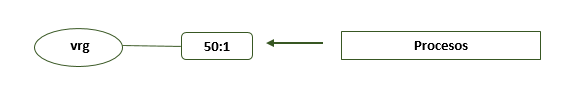
\includegraphics[width=0.75\linewidth]{Imagenes/ima12} 

}

\caption{VRG}\label{fig:unnamed-chunk-40}
\end{figure}

El requerimiento de la VRG \emph{``Informe Revisión por la Dirección''} que se alimenta con todos los
procesos de la Universidad, está siendo parciamente satisfecho para sus usuarios, eso debido a
que no siempre envían la información de manera completa y oportuna, por no contar con un
sistema implementado.

\begin{figure}

{\centering 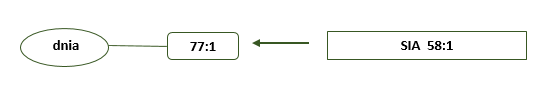
\includegraphics[width=0.75\linewidth]{Imagenes/ima13} 

}

\caption{DNIA}\label{fig:unnamed-chunk-41}
\end{figure}

El requerimiento de la DNIA está completamente satisfecho.

\begin{figure}

{\centering 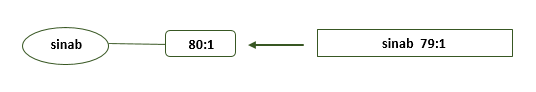
\includegraphics[width=0.75\linewidth]{Imagenes/ima14} 

}

\caption{SINAB}\label{fig:unnamed-chunk-42}
\end{figure}

El SINAB reporta un requerimiento de información y este se encuentra completamente satisfecho.

\begin{figure}

{\centering 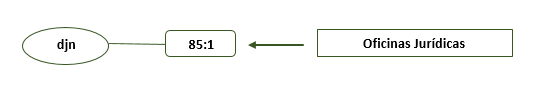
\includegraphics[width=0.75\linewidth]{Imagenes/ima15} 

}

\caption{DJN}\label{fig:unnamed-chunk-43}
\end{figure}

El DJN presenta un requerimiento que está completamente satisfecho.

\begin{figure}

{\centering 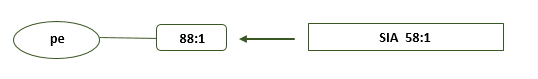
\includegraphics[width=0.75\linewidth]{Imagenes/ima16} 

}

\caption{PE}\label{fig:unnamed-chunk-44}
\end{figure}

El requerimiento del PE está completamente satisfecho.

\begin{figure}

{\centering 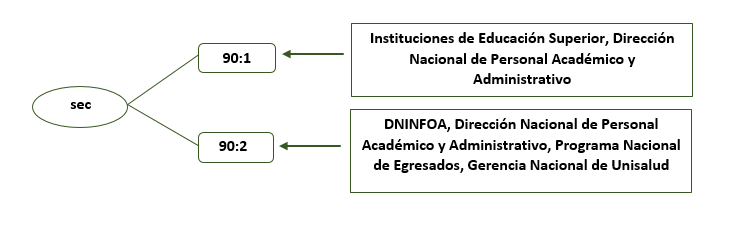
\includegraphics[width=0.75\linewidth]{Imagenes/ima17} 

}

\caption{SEC}\label{fig:unnamed-chunk-45}
\end{figure}

Los requerimientos del SEC se encuentran completamente satisfechos.

\begin{figure}

{\centering 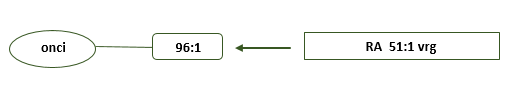
\includegraphics[width=0.75\linewidth]{Imagenes/ima18} 

}

\caption{ONCI}\label{fig:unnamed-chunk-46}
\end{figure}

La ONCI cuenta con un requerimiento de información que se encuentra completamente
satisfecho.

\hypertarget{insumo-complementario-para-identificaciuxf3n-de-necesidades-relacionadas-con-el-proceso-estaduxedstico}{%
\subsection{Insumo complementario para identificación de necesidades relacionadas con el proceso estadístico}\label{insumo-complementario-para-identificaciuxf3n-de-necesidades-relacionadas-con-el-proceso-estaduxedstico}}

En aras de vincular dentro del diagnóstico y mejoramiento de los procesos estadísticos la
participación de los gestores y generadores de información en cada una de las dependencias
vinculadas en la construcción del Plan Estadístico Institucional, se construyó y aplicó un formato
de encuesta semi -estructurada que buscaba indagar sobre aspectos que no se indagaron en los
formatos de caracterización de ofertas y demandas de información estadística. Los resultados de
la aplicación de dicho instrumento se consolidan en este apartado.

\hypertarget{encuesta-de-percepciuxf3n-sobre-el-proceso-estaduxedstico-y-el-manejo-de-informaciuxf3n-estaduxedstica}{%
\subsubsection{Encuesta de percepción sobre el proceso estadístico y el manejo de información estadística}\label{encuesta-de-percepciuxf3n-sobre-el-proceso-estaduxedstico-y-el-manejo-de-informaciuxf3n-estaduxedstica}}

\textbf{\emph{1. Descripción de los entrevistados:}}

Las personas entrevistadas son los funcionarios encargados del manejo de información estadística,
y que fueron delegados para participar en la construcción del Plan Estadístico de la Universidad. En
esta encuesta participaron 31 funcionarios, 20 de planta, 1 provisional y 9 contratistas.

De acuerdo a los niveles de formación indicados en la encuesta, se identificó que 19 de los
funcionarios tienen título de posgrado, 10 pregrado, un tecnólogo, y una persona con título de
secundaria.

Tres funcionarios llevan a cargo de la información estadística menos de 6 meses, otros cinco, entre 6
meses y un año, cuatro funcionarios, entre uno y tres años, nueve funcionarios, de tres a diez años y cuatro funcionarios llevan más de diez años.

En relación a las herramientas que utilizan para la construcción y visualización de la información
estadística, 26 de los funcionarios utiliza Excel, 6 utilizan SQL, 4 Tableau, 3 SPSS y uno utiliza R. 4 de
los funcionarios reportaron utilizar otros programas.

\textbf{\emph{2. Percepción sobre el proceso estadístico y el manejo de información estadística:}}

\begin{figure}
\centering
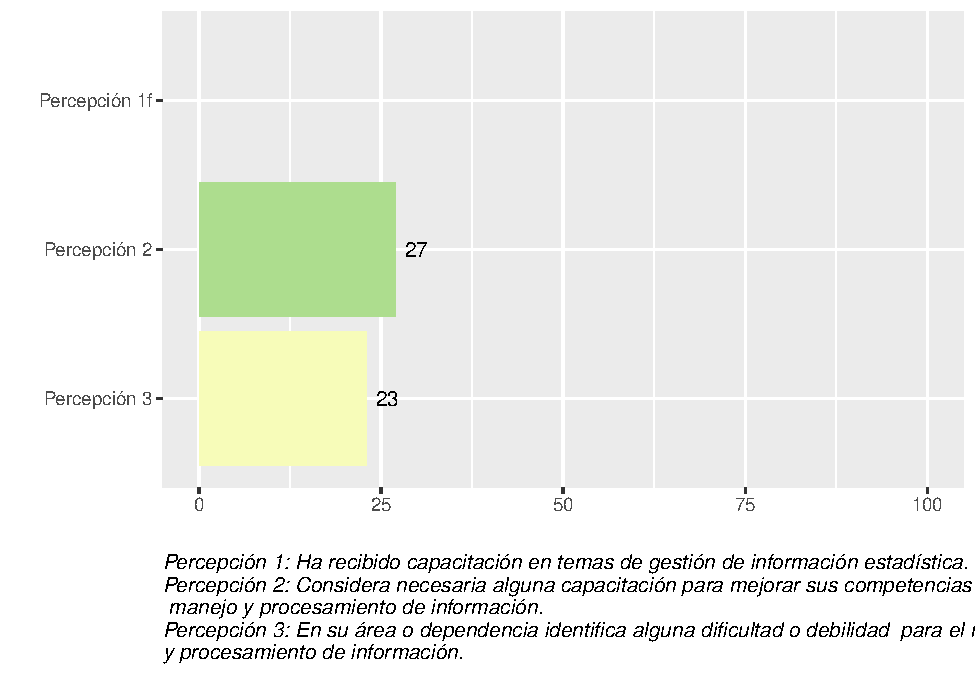
\includegraphics{Plan-Estadistico_files/figure-latex/unnamed-chunk-48-1.pdf}
\caption{\label{fig:unnamed-chunk-48}Habilidades y capacitaciones}
\end{figure}

De los 31 funcionarios entrevistados, 8 han recibido algún tipo de capacitación en gestión de información estadística, los temas en los que se han capacitado son:

\begin{itemize}
\tightlist
\item
  Business Intelligence Analytical
\item
  Formación en indicadores de gestión
\item
  Análisis de datos
\item
  Manejo de SAS
\end{itemize}

Aún así, 27 de los entrevistados, que corresponden al 87\%, consideran que es necesario mejorar las competencias en esta área, 23 de ellos identifican dificultades en este mismo asunto en las áreas o dependencias en las que laboran. Entre las capacitaciones solicitadas, mencionan: Manejo de software (12), producción de estadísticas e indicadores (5), Evaluación de calidad de la información estadística (4), Análisis de datos (3), Gestión de la información (3), Creación y procesamiento de bases de datos (3), Formulación de indicadores (3), Big data (2), Metodologías de análisis estadístico (2), Presentación de resultados estadísticos (2), Acceso a fuentes de información de la UNAL (1) y Business Intelligence (1).

\begin{figure}
\centering
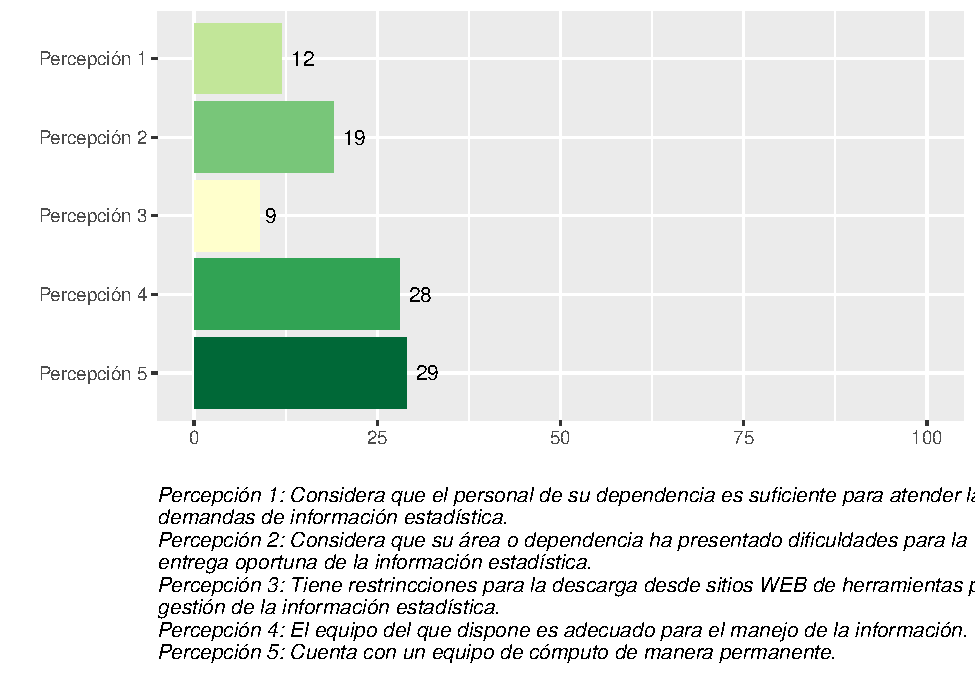
\includegraphics{Plan-Estadistico_files/figure-latex/unnamed-chunk-50-1.pdf}
\caption{\label{fig:unnamed-chunk-50}Recursos físicos, humanos tecnológicos}
\end{figure}

Al analizar los recursos con los que se cuenta para el
manejo de información, se identifica por parte de los funcionarios que los principales inconvenientes son que falta personal para atender las demandas de
información, ya que solo 12 de los 31 consideran que el personal es suficiente. De igual forma, 19 identifican dificultades para la entrega oportuna de información estadística, problema que puede estar
relacionado con el anterior. En cuanto a equipos de cómputo no se observan muchos inconvenientes, 29 cuentan con equipos permanentes y 28 consideran que su equipo es adecuado para el manejo de información. Nueve (9) funcionarios reportaron que tienen restricciones de acceso a páginas web que consideran que son necesarias para la gestión de la información estadística que tienen a cargo.

\textbf{\emph{3. Percepción sobre la producción estadística:}}

\begin{figure}
\centering
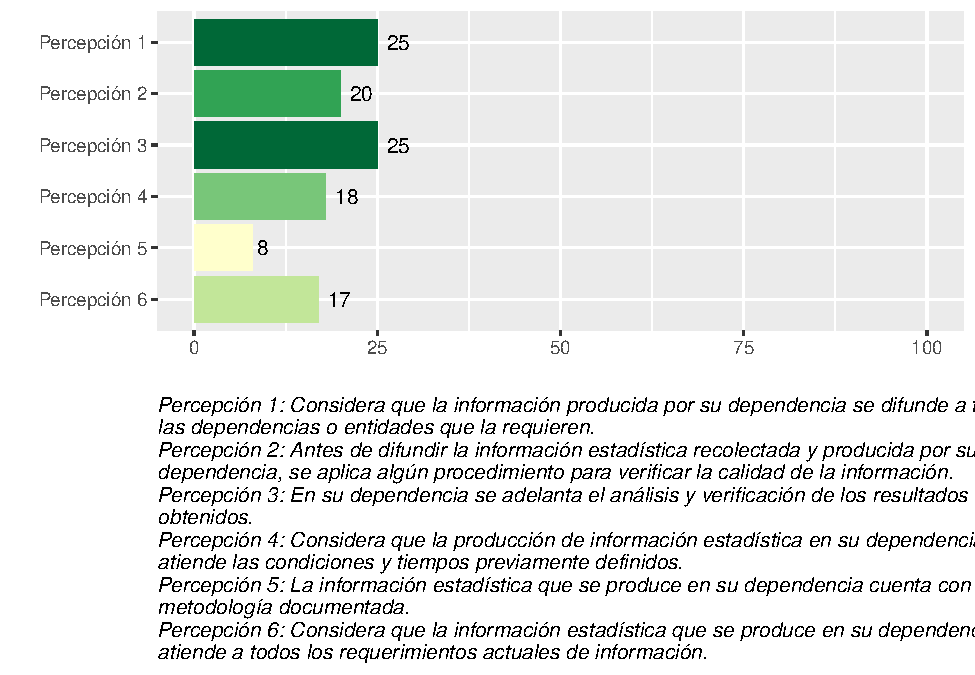
\includegraphics{Plan-Estadistico_files/figure-latex/unnamed-chunk-52-1.pdf}
\caption{\label{fig:unnamed-chunk-52}Manejo y aprovechamiento de la información producida}
\end{figure}

En relación al proceso estadístico desarrollado en las dependencias de la Universidad, desde la perspectiva de los funcionarios, 25 consideran que la información se difunde a los usuarios que la requieren, aunque al preguntarles si consideran que se están atendiendo todos los requerimientos, solo 17 consideran que esto es así.

En relación a controles de calidad, 20 mencionan que se realizan procedimientos para verificar la calidad de la información recolectada y producida y 25 que se realiza verificación de los resultados obtenidos, aunque tan solo 8 reportan que se cuenta con metodología documentada. Dieciocho (18) mencionan que la información atiende las condiciones y tiempos definidos.

\textbf{Comentarios y sugerencias adicionales de los funcionarios}

Nueve de los funcionarios realizaron comentarios adicionales a lo indagado, la síntesis se presenta a continuación:

\begin{itemize}
\item
  Consideran que debe existir un funcionario capacitado
  para manejo de información estadística.
\item
  Dado que no se tiene información organizada se hace
  dispendioso entregar información a tiempo y luego el
  análisis requerido.
\item
  Desde el proceso de admisiones se obtienen datos,
  cifras que pueden alimentar otras dependencias para
  generar estadísticas.
\item
  El manejo de la información estadística requiere de
  un enfoque institucional para alinear a toda la
  dirección de la UNAL con sus dependencias adscritas en
  la forma en que se recolecta y organiza la
  información.

  NOTA: Es importante en la primera construcción no
  mezclar los indicadores de calidad con el tema de
  estadísticas.
\item
  Es importante poder acceder a la
  información estadística en línea, en tiempo real con
  actualización automática y bajo estándares
  entendibles y accesibles rápidamente.
\item
  Es necesario establecer los indicadores básicos lo
  más pronto posible; o por lo menos una metodología estandarizada y articulada
  con las diferentes facultades, revisión de los que existe. Se debe establecer un papel más activo a cada una de las facultades, institutos y dependencias; tener en cuenta sus necesidades básicas de información.
\item
  Las bases de datos que están almacenadas muchas veces
  no son compatibles con las sedes o no se comparte con
  las unidades administrativas y se genera duplicidad
  de datos en las bases de la Universidad.
\item
  Se requiere que sean muy puntuales para aplicar los
  lineamientos y métodos para la aplicación de la
  información.
\item
  Sería importante desde la DNPE establecer lineamientos
  estandarizados para trabajar la planeación
  estratégica y operativa, así como para la
  documentación y evaluación de indicadores.
\end{itemize}

\hypertarget{formulaciuxf3n-del-componente-estratuxe9gico-del-plan-estaduxedstico}{%
\chapter{Formulación del componente estratégico del Plan Estadístico}\label{formulaciuxf3n-del-componente-estratuxe9gico-del-plan-estaduxedstico}}

En esta apartado se consolidan las propuestas de corto, mediano y largo plazo, que surgen como resultado de los hallazgos obtenidos del diagnóstico de la información estadística disponible, de la consolidación de requerimientos de información o demandas insatisfechas de información y de las necesidades explicitas de funcionarios responsables del manejo de información estadística en sus áreas respectivas.

El conjunto de acciones y recomendaciones orientadas hacia el mejoramiento de los procesos estadísticos internos se circunscriben en el siguiente Plan de Acción.

\hypertarget{plan-de-acciuxf3n-para-el-fortalecimiento-estaduxedstico-institucional}{%
\section{Plan de acción para el fortalecimiento estadístico institucional}\label{plan-de-acciuxf3n-para-el-fortalecimiento-estaduxedstico-institucional}}

Para facilitar la organización, focalización y comprensión de las acciones de mejoramiento consignadas, se proponen dos elementos: en primer lugar, la construcción de una matriz de intervención institucional orientada hacia los procesos estadísticos adoptados para la generación de información estadística (operaciones estadísticas) y en segundo lugar un conjunto de recomendaciones y acciones que surgen del inventario y revisión de registros administrativos RRAA con potencial uso estadístico.

Dentro de la consolidación de este conjunto de acciones y recomendaciones se consideraron algunos postulados generales, denominados lineamientos orientadores, que limitan el alcance de las acciones e intervenciones propuestas y de unos principios rectores de la actividad estadística en la Universidad, que determinan las pautas básicas a seguir en los procesos de consolidación, procesamiento, análisis, difusión y uso de la información estadística institucional.

\hypertarget{lineamientos-orientadores}{%
\subsection{Lineamientos orientadores}\label{lineamientos-orientadores}}

\begin{itemize}
\item
  \textbf{Lineamiento N°1:} Concreción del concepto de valor público en la construcción de estadísticas institucionales. Se refiere a propender que la generación de estadísticas permita adelantar la evaluación y seguimiento a los resultados institucionales alcanzados (medibles) para dar respuesta a las necesidades o demandas sociales, resultados asociados a los cambios sociales producidos por la acción institucional y por las actividades y productos entregados por las diferentes dependencias de la Universidad Nacional (BID, 2015). Puntualmente haciendo de la información un elemento articulador de las dimensiones del Modelo Integrado de Planeación y Gestión, en la medida que le permiten a la vinculación de la institución y su entorno y le facilita la ejecución de sus operaciones internas. Se hace énfasis en el enfoque transversal de la Información y la comunicación frente a los demás componentes del Modelo, pues permite ampliar y profundizar en el uso y aprovechamiento de la información para los procesos internos de la Universidad (toma de decisiones, elaboración de política pública, entre otros), así como la interacción con la comunidad (grupos de valor y grupos de interés).
\item
  \textbf{Lineamiento N°2:} Reconocimiento del valor estratégico de la información y promoción del aprovechamiento de datos, mediante el desarrollo de las condiciones para que los datos generados por diferentes fuentes, sean gestionados como activos que pueden generar valor social y económico en cuanto permiten brindar respuestas efectivas y útiles frente a las necesidades de los diferentes actores institucionales.
\item
  \textbf{Lineamiento N°3:} Adopción de las regulaciones y lineamientos del Sistema Estadístico Nacional en lo referente a las fases y caracterización de los procesos estadísticos institucionales y cuyo objeto es fortalecer la capacidad institucional para producir información de calidad y orientar a las entidades en las actividades requeridas para la generación de estadísticas dependiendo las diferentes fuentes de información (censos, por muestreo o a partir de registros
  administrativos).
\end{itemize}

\hypertarget{principios-para-la-actividad-estaduxedstica-en-la-universidad-nacional-de-colombia}{%
\subsection{Principios para la actividad estadística en la Universidad Nacional de Colombia}\label{principios-para-la-actividad-estaduxedstica-en-la-universidad-nacional-de-colombia}}

Con base en las discusiones y mesas de trabajo realizadas para la formulación del Plan Estadístico de la Universidad Nacional de Colombia, se consideró pertinente adoptar y asumir unos principios básicos para el procesamiento, generación, análisis y difusión de estadísticas, tomando como base los propuestos en otras Entidades, como el Instituto Nacional de Estadística y Geografía de México, y el Sistema Estadístico Nacional. Los siguientes son los principios definidos:

\begin{itemize}
\item
  \textbf{Confidencialidad:} Se debe garantizar que los datos obtenidos para la producción de estadísticas de las distintas fuentes, ya sean personas naturales o jurídicas, deben ser estrictamente confidenciales y utilizarse exclusivamente para fines estadísticos.
\item
  \textbf{Interpretabilidad:} Para la correcta interpretación de los datos, se debe presentar información referenciada sobre los conceptos, métodos y procedimientos estadísticos utilizados.
\item
  \textbf{Pertinencia:} Debe existir una clara relación entre la información estadística producida y los objetivos en los que se enmarca esta.
\item
  \textbf{Transparencia:} Condición bajo la cual se pone a disposición de los usuarios, los metadatos que permiten conocer el desarrollo de la operación estadística.
\item
  \textbf{Rigurosidad:} Consiste en la aplicación sistemática de los principios, métodos y procedimientos generalmente aceptados por la técnica y la ciencia estadística.
\item
  \textbf{Eficiencia:} Es la relación entre el valor de los resultados de la actividad estadística y el costo generado para obtenerlos, teniendo en cuenta el uso adecuado de los recursos disponibles.
\item
  \textbf{Oportunidad:} Se refiere al tiempo que transcurre entre la ocurrencia del fenómeno de estudio y la publicación o difusión de la información estadística, de tal forma que sea útil para la toma de decisiones.
\end{itemize}

\hypertarget{estructura-de-la-matriz-de-intervenciuxf3n}{%
\subsection{Estructura de la matriz de intervención}\label{estructura-de-la-matriz-de-intervenciuxf3n}}

La matriz de intervención es un recurso creado para organizar de manera coherente las acciones y recomendaciones que propone el Plan Estadístico Institucional, y son usadas en el diagnostico y evaluación.

\begin{itemize}
\item
  \textbf{Línea estratégica:} En este componente se establece una asociación entre las fases del proceso estadístico (Detección y análisis de requerimientos, Ejecución, Análisis, Difusión) y la cadena de valor (insumos, procesos, productos y resultados)utilizada como herramienta principal para representar las intervenciones públicas (DNP, 2015a) o las actividades gubernamentales (OCDE, 2009); la asociación se sintetiza en tres grandes procesos en los que se orienta y soporta la actividad estadística en general: Programación Estadística (¿qué?,¿ cuándo?, ¿quién? y ¿dónde? se produce la información estadística?), producción estadística (¿cómo se produce? y ¿cuáles son lineamientos de Aseguramiento de la calidad estadística y Regulación estadística?), Usabilidad y aprovechamiento de la información generada (¿Para qué?) y un cuarto proceso se refiere a las adaptaciones institucionales o capacidades para entronizar en funcionarios y dependencias una visión estratégica de la información estadística institucional este proceso se define como cultura estadística.

  Con esta organización se busca que se identifiquen y
  focalicen las intervenciones institucionales en el
  proceso en las cual se presenten sugerencias o
  recomendaciones de mejora y se eviten las
  intervenciones muy generales que pretendan atender
  todas las componentes de la actividad estadística
  simultáneamente.
\item
  \textbf{Aspecto susceptible de mejora:} Este componente de la matriz de acción describe el conjunto de hallazgos y elementos que requieren atención en términos de fortalecimiento estadístico. Sintetiza las dificultades u oportunidades de mejora, identificadas con la revisión y análisis de información adelantado en el desarrollo del proyecto, en otros términos, referencia los errores recurrentes en la producción, consolidación, procesamiento y análisis de información estadística o que demuestran desconocimiento; además se incluyen los aportes, recomendaciones o solicitudes explicitas consolidadas mediante encuestas y entrevistas con los funcionarios y que evidencian necesidades en materia de producción o gestión de la información estadística en la Universidad.
\item
  \textbf{Estrategia:} Se refiere a las líneas generales de Intervención que buscan mejorar la gestión, producción, análisis y difusión de información estadística de carácter estratégico y que abren paso a una sucesión de acciones que tienen como propósito la consecución de un determinado objetivo.
\item
  \textbf{Acciones puntuales de mejora:} Recomendaciones de acción propuestas con base en el conjunto de estrategias definidas. Su importancia radica en la conveniencia de precisar acciones concretas que permitan avanzar en la atención oportuna de cada uno de los aspectos susceptibles de mejora.
\item
  \textbf{Metas:} Hacen referencia al desempeño esperado en la materialización de cada una de las acciones de fortalecimiento propuestas. Desde esta perspectiva, permite medir el cumplimiento del plan de acción propuesto.
\item
  \textbf{Indicador:} En este contexto se refiere a la unidad que permite medir o comparar los resultados efectivamente obtenidos, en la ejecución de cada una de las acciones propuestas en el plan de acción. Permite conocer un ``valor'' de comparación referido a cada META asociada.
\item
  \textbf{Responsable:} Es un componente esencial de la matriz en la medida que se define quién o quiénes son los responsables de promover, socializar, implementar y hacer seguimiento de cada una de las acciones de fortalecimiento estadístico propuestas en el Plan de Acción.
\item
  \textbf{Tiempo requerido:} Es una dimensión esencial en un Plan de Acción, y en este caso se refiere al periodo definido para la implementación de cada una de las acciones propuestas.
\item
  \textbf{Ámbitos:} Hace referencia al alcance de la intervención o de la acción institucional, en este componente se identifica específicamente el actor objeto de intervención, es decir, hacia quién debe orientarse las acciones de fortalecimiento estadístico. En ese sentido, se delimitan las acciones enfocadas hacia el individuo, es decir, aquellas que consideran al funcionario como la unidad de intervención e implementación de la acción propuesta. Por otro lado, se organizan las acciones que tienen como objeto de intervención cada una de las dependencias que conforman el nivel central de la Universidad Nacional y que tienen en su haber la producción o utilización de información estadística Estratégica. Finalmente, se conforma un conjunto con las acciones de mejora de carácter general para la Universidad, es decir, aquellas acciones que implican cambios o ajustes a nivel global para garantizar o mejorar la producción estadística en condiciones de calidad, oportunidad y confiabilidad.
\item
  \textbf{Priorización:} De acuerdo con la magnitud de la recomendación y la disponibilidad de recursos para asumir su implementación es necesario establecer un orden jerárquico a las acciones propuestas, se propone entonces la siguiente calificación: alta si el nivel de atención e implementación es imperativo, media si las acciones se pueden implementar de manera progresiva y baja si es posible postergar en alguna medida su implementación o si la no implementación no afecta de manera significativa el proceso de fortalecimiento estadístico.

  Si bien en la matriz, la lectura se debe hacer de
  forma horizontal, el esquema analítico para la
  formulación de las acciones atiende cierta
  verticalidad, partiendo desde los ejes de
  intervención hasta llegar a la definición de
  responsables y tiempos requeridos para su ejecución.
\end{itemize}

\begin{figure}

{\centering 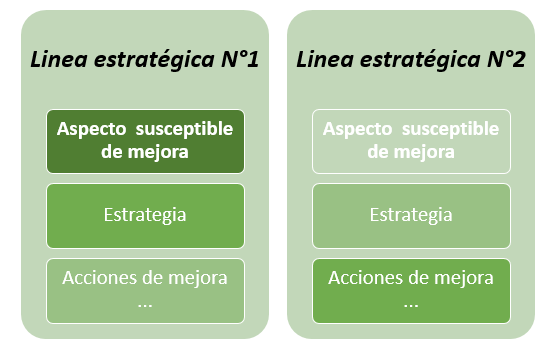
\includegraphics[width=0.6\linewidth]{Imagenes/diagrama} 

}

\caption{Estructura de la matriz}\label{fig:unnamed-chunk-53}
\end{figure}

Este modelo requiere como complemento a la formulación de las acciones propuestas, la socialización, validación y aprobación por parte de los responsables de los procesos, con lo cual se busca que los funcionarios delegados de las dependencias y el equipo técnico del proyecto, acuerden para cada acción propuestas a los siguientes elementos: metas, tiempo y recursos requeridos para su implementación, responsables en el desarrollo e implementación de las acciones y se define el nivel de importancia o prioridad que se asignaría a cada una.

Con esta estructura se busca facilitar la comprensión y operacionalización del conjunto de recomendaciones, sugerencias y acciones contenidas en este documento, además, ofrece la posibilidad de ordenar y priorizar acciones de acuerdo a las demandas más relevantes en sus procesos de producción y gestión de información estadística.

\hypertarget{marco-conceptual-de-la-matriz-de-intervenciuxf3n}{%
\subsection{Marco conceptual de la matriz de intervención}\label{marco-conceptual-de-la-matriz-de-intervenciuxf3n}}

En este apartado se integran los principales conceptos que orientan la estructura de la matriz y las acciones de intervención propuestas.

\hypertarget{planificaciuxf3n-estaduxedstica}{%
\subsubsection{Planificación estadística}\label{planificaciuxf3n-estaduxedstica}}

La Planificación Estadística es un proceso técnico, dinámico y permanente que define, organiza y prioriza las estadísticas requeridas para la toma de decisiones\footnote{\protect\hyperlink{ref-BibEntry2021May}{{``{Aspectos generales}''}} (\protect\hyperlink{ref-BibEntry2021May}{2021})}. Facilita la coordinación y regulación de la actividad estadística para optimizar, en un tiempo determinado y con unos recursos establecidos, la gestión, utilidad y aprovechamiento de esta información.

Para el caso particular de la Universidad, la planificación estadística establece el conjunto de procesos necesarios que permiten: Conocer, diagnosticar y organizar la actividad estadística y establecer lineamientos para su fortalecimiento; identificar y priorizar la información estadística requerida para la formulación y el diseño de políticas, planes, proyectos; determinar las necesidades de información estadística y desarrollar un plan para resolver las necesidades y limitaciones de información; contribuir al uso eficiente de los recursos financieros, tecnológicos y humanos dirigidos hacia la actividad estadística; facilitar la toma de decisiones, el seguimiento, monitoreo y evaluación de las políticas, planes y programas institucionales; facilitar la articulación entre productores y usuarios fortaleciendo su comunicación y coordinación en cuanto a la producción y el manejo de la información estadística.

En ese sentido el objetivo de las acciones planteadas en este apartado, es: ``Promover la definición, organización, priorización y producción de estadísticas institucionales requeridas para la toma de decisiones.''

Como resultados de la revisión de la información estadística identificada y documentada por los funcionarios en la construcción del Plan Estadístico Institucional, se identificó un conjunto de aspectos en términos de planificación estadística, susceptibles de mejorar.

\hypertarget{aseguramiento-de-la-calidad-estaduxedstica}{%
\subsubsection{Aseguramiento de la Calidad Estadística}\label{aseguramiento-de-la-calidad-estaduxedstica}}

Es el instrumento mediante el cual se asegura la calidad del proceso estadístico dentro del marco de los \emph{``Principios Fundamentales de las Estadísticas Oficiales de Naciones Unidas''} y de los criterios de calidad sugeridos por el DANE como pertinentes para cumplir con los requisitos y necesidades de los usuarios, y así contribuir a la credibilidad, confiabilidad y transparencia en la producción de información estadística (DANE, 2015). Establece un conjunto de procedimientos necesarios, orientados a garantizar que un producto o servicio cumpla con los estándares de calidad de la información.

Acorde con estas premisas, el objetivo de esta sección es adelantar recomendaciones en torno al proceso de producción de información estadística estratégica en la Universidad Nacional, analizando las principales variables que permiten el aseguramiento de su calidad.

El objetivo fundamental de las acciones incluidas en este apartado es:

\emph{``Asegurar la calidad de los procesos estadísticos adelantados por las áreas y dependencias del nivel central de la Universidad Nacional, de acuerdo a los estándares nacionales e internacionales, de manera que las estadísticas generadas cuenten con credibilidad, confiabilidad y transparencia en su producción.''}

\hypertarget{regulaciuxf3n-estaduxedstica}{%
\subsubsection{Regulación Estadística}\label{regulaciuxf3n-estaduxedstica}}

Es un instrumento mediante el cual se adoptan un conjunto de buenas prácticas, normas y estándares estadísticos. Su implementación, permite la armonización, comparabilidad, agregabilidad, calidad e integración de las estadísticas oficiales en el país, dentro del marco de los Principios Fundamentales de las Estadísticas Oficiales de la Organización de las Naciones Unidas (ONU).

La regulación estadística genera las reglas que serán aplicables al conjunto de procesos, procedimientos, métodos y técnicas para el diseño, la recolección, el tratamiento, el análisis, la actualización, la organización, el procesamiento, la integración, la compilación y la conservación de datos e información de carácter estadístico (DANE,2015).

Como resultado de la adopción de los principios de la regulación estadística se espera cumplir con el objetivo fundamental de mejorar los procesos, procedimientos y métodos utilizados en la elaboración de las estadísticas institucionales; con estos elementos se fortalece, la comparabilidad, la calidad, la credibilidad y la integridad de las estadísticas que produce la Universidad y se contribuye a la identificación e implementación de las buenas prácticas y los estándares para la producción estadística.

\hypertarget{cultura-estaduxedstica}{%
\subsubsection{Cultura Estadística}\label{cultura-estaduxedstica}}

En este eje se incluyen los elementos relacionados con las prácticas cotidianas en el desarrollo de actividades de gestión, manejo, producción y difusión de información estadística, tanto de los funcionarios como de las dependencias que componen la Universidad. En particular se refiere a aspectos relacionados con dos componentes interrelacionados:

\begin{itemize}
\item
  Capacidad para interpretar y evaluar críticamente la
  información estadística, los argumentos apoyados en
  datos o los fenómenos que los funcionarios pueden
  encontrar en diversos ámbitos de la Universidad.
\item
  Capacidad para discutir, soportar y difundir sus
  opiniones respecto a tales informaciones
  estadísticas cuando sea relevante, con argumentos y
  procesos validados que se ven directamente
  relacionados con:

  \begin{itemize}
  \item
    Conocimientos y destrezas de los componentes
    básicos conceptual y procedimental de la
    estadística. Según Moreno (1998).
  \item
    El razonamiento estadístico que incluye según
    Wild y Pfannkuch (1999) como componentes
    fundamentales:

    \begin{itemize}
    \item
      Reconocer la necesidad de los datos.
    \item
      Transnumeración o la comprensión que puede
      surgir al cambiar la representación de los
      datos.
    \item
      Percepción de la variación. La recogida
      adecuada de datos y los juicios correctos a
      partir de los mismos requieren la
      comprensión de la variación que hay y se
      transmite en los datos.
    \item
      \emph{Intuiciones:} Al enfrentarnos a las
      situaciones cotidianas y tareas
      profesionales en que es preciso tomar
      decisiones basadas en la evaluación de
      probabilidades inconscientemente podemos
      suprimir una parte de la información y
      producir decisiones sesgadas.
    \item
      \emph{Actitudes:} La cultura no es solamente conocimiento y capacidad. La parte emocional--sentimientos, valores, actitudes son también componentes importantes.
    \end{itemize}
  \end{itemize}
\end{itemize}

\hypertarget{suxedntesis-de-la-matriz-de-intervenciuxf3n}{%
\subsection{Síntesis de la matriz de intervención}\label{suxedntesis-de-la-matriz-de-intervenciuxf3n}}

En este apartado se presentan de manera sintética las líneas estratégicas, así como los objetivos del Plan Estadístico Institucional las cuales se desarrollarán de manera precisa en el \protect\hyperlink{Cap6}{Capítulo 6}.

\begin{itemize}
\item
  \textbf{Línea estratégica 1:} LINEAMIENTOS CONCEPTUALES Y METODOLÓGICOS

  \begin{itemize}
  \item
    \textbf{Objetivo 1.} Producir los lineamientos conceptuales que orienten la actividad estadística en la Universidad.
  \item
    \textbf{Objetivo 2.} Establecer los instrumentos metodológicos que apoyen el desarrollo de la actividad estadística en la Universidad.
  \end{itemize}
\item
  \textbf{Línea estratégica 2:} PRODUCCIÓN ESTADÍSTICA

  \begin{itemize}
  \item
    \textbf{Objetivo 1.} Establecer y adoptar los lineamientos del proceso estadístico para la generación de estadísticas estratégicas institucionales.

    \begin{itemize}
    \tightlist
    \item
      \textbf{Objetivo 2.} Fortalecer la gestión estadística institucional
    \end{itemize}
  \end{itemize}
\item
  \textbf{Línea estratégica 3:} GESTIÓN DE LAS CAPACIDADES TÉCNICAS Y TECNOLÓGICAS PARA LA PRODUCCIÓN ESTADÍSTICA

  \begin{itemize}
  \tightlist
  \item
    \textbf{Objetivo 1.} Fortalecer las capacidades técnicas y tecnológicas para la gestión de la información estadística institucional (disposición de hardware y adquisisicón y dominio de software).
  \end{itemize}
\item
  \textbf{Línea estratégica 4:} CULTURA ESTADÍSTICA

  \begin{itemize}
  \item
    \textbf{Objetivo 1.} Promover la difusión y conocimiento de la información estadística estratégica institucional.
  \item
    \textbf{Objetivo 2.} Promover el uso y aprovechamiento de los datos, estadísticas e indicadores como activo estratégico institucional.
  \end{itemize}
\end{itemize}

\hypertarget{Cap6}{%
\chapter{Plan de acción}\label{Cap6}}

\hypertarget{luxednea-estratuxe9gica-i-lineamientos-conceptuales-y-metodoluxf3gicos}{%
\subsection{\texorpdfstring{\emph{Línea Estratégica I:} Lineamientos conceptuales y metodológicos}{Línea Estratégica I: Lineamientos conceptuales y metodológicos}}\label{luxednea-estratuxe9gica-i-lineamientos-conceptuales-y-metodoluxf3gicos}}

\begin{itemize}
\item
  \emph{Objetivo específico 1:}

  Construir \textbf{LINEAMIENTOS CONCEPTUALES} que orienten
  la actividad estadística en la Universidad y que aporten al fortalecimiento de la producción estadística a nivel nacional e internacional.

  \begin{itemize}
  \item
    \emph{Acción 1:}

    \textbf{Desarrollar elementos conceptuales} que sirvan de referencia para la actividad estadística a nivel institucional y en el contexto nacional e internacional.

    \begin{itemize}
    \item
      \emph{Línea de base:}

      Libro: \href{https://estadisticaun.github.io/L_Conceptual/}{Gestión de la información cuantitativa en las universidades}.
    \item
      \emph{Comentarios:}

      Tener en cuenta dentro del estado del arte que ya se cuenta con un documento inicial de marco conceptual, ¿se podría cambiar la estrategía a socializar?
    \end{itemize}
  \item
    \emph{Acción 2:}

    Estudiar el \textbf{uso potencial y alcance de técnicas contemporáneas} para el análisis de la información estadística institucional con propósitos explicativos, evaluativos o predictivos.

    \begin{itemize}
    \item
      \emph{Comentario Nivel 1:}

      Técnicas contemporáneas: minería o analítica de datos, estadística, ciencia de los datos, big data, inteligencia de negocios.
    \end{itemize}
  \item
    \emph{Acción 3:}

    \textbf{Establecer el marco conceptual} y alcance para el monitoreo y seguimiento a planes, programas y proyectos institucionales a través de la construcción de indicadores desde una perspectiva cuantitativa.

    \begin{itemize}
    \item
      \emph{Comentarios:}

      Es importante desarrollarlo en el Plan II, teniendo en cuenta el proceso de formulación y desarrollo del PLEI.
    \end{itemize}
  \item
    \emph{Acción 4:}

    \textbf{Aportar a la definición de los elementos conceptuales y metodológicos que sirvan de referencia} para el desarrollo de evaluaciones a políticas, planes y proyectos institucionales desde una perspectiva cuantitativa.

    \begin{itemize}
    \item
      \emph{Comentarios:}

      Es importante acotar los documentos conceptuales y metodológicos de acuerdo con el uso de la información estadística (perspectiva cuantitativa).

      \begin{itemize}
      \item
        \emph{Acción nivel 2:}

        Realizar un estado del arte de las técnicas y metodologías empleadas para la evaluación de las políticas en el ámbito de la educación.
      \end{itemize}
    \end{itemize}
  \end{itemize}
\item
  \emph{Objetivo específico 2:}

  Definir y construir \textbf{INSTRUMENTOS METODOLÓGICOS} que apoyen
  el desarrollo de la actividad estadística.

  \begin{itemize}
  \item
    \emph{Acción 1:}

    \textbf{Definir y construir una guía metodológica} para el desarrollo y gestión de las \textbf{estadísticas oficiales} institucionales.
  \item
    \emph{Acción 2:}

    \textbf{Definir y construir una guía metodológica} que orienten la construcción de \textbf{indicadores de los procesos} en la Universidad.

    \begin{itemize}
    \item
      \emph{Acción nivel 2:}

      Actualizar la guía para la construcción de indicadores de proceso.
    \end{itemize}
  \item
    \emph{Acción 3:}

    Definir y construir una \textbf{guía metodológica para el seguimiento y monitoreo} a través de indicadores de planes, programas y proyectos institucionales.
  \item
    \emph{Acción 4:}

    Aportar al desarrollo de un \textbf{documento metodológico para la evaluación} de políticas, planes, programas y proyectos institucionales.
  \end{itemize}
\end{itemize}

\hypertarget{luxednea-estratuxe9gica-ii-producciuxf3n-estaduxedstica}{%
\subsection{\texorpdfstring{\emph{Línea Estratégica II:} Producción estadística}{Línea Estratégica II: Producción estadística}}\label{luxednea-estratuxe9gica-ii-producciuxf3n-estaduxedstica}}

\begin{itemize}
\item
  \emph{Objetivo específico 3:}

  Definir, adoptar o adaptar un marco orientador para la definición del \textbf{PROCESO ESTADÍSTICO} requerido para la producción de estadísticas oficiales.
\item
  \emph{Acción 1:}

  Definir y adptar el \textbf{marco orientador} para la implementación del \textbf{proceso estadístico} a nivel institucional.

  \begin{itemize}
  \item
    \emph{Línea de base:}

    \href{https://www.dane.gov.co/files/sen/normatividad/NTC-Proceso-Estadistico-PE-1000-2020.pdf}{Norma Técnica de Calidad del Proceso Estadístico - NTCPE 1000}.
  \end{itemize}
\item
  \emph{Acción 2:}

  \textbf{Implementar y documentar el proceso estadístico} que soporta las operciones estadísticas requeridas para la producción de la información estadística oficial.
\item
  \emph{Objetivo específico 4:}
\end{itemize}

Fortalecer los \textbf{mecanismos de construcción y disposición} de las \textbf{ESTADÍSTICAS E INDICADORES} oficiales institucionales.

\begin{itemize}
\item
  \emph{Acción 1:}

  \textbf{Aumentar gradualmente,} a través de un ejercicio de priorización, la producción de \textbf{estadísticas e indicadores oficiales institucionales}.

  \emph{Acciones nivel 2:}

  \begin{itemize}
  \tightlist
  \item
    Definir un mecanismo institucional para la priorización en la construcción y publicación de estadísticas oficiales.
  \end{itemize}
\item
  \emph{Acción 2:}

  Fortalecer los mecanismos de \textbf{difusión y comunicación} de las estadísticas oficiales e indicadores institucionales.

  \emph{Acciones nivel 2:}

  \begin{itemize}
  \tightlist
  \item
    Fortalecer, de manera continua, la página web de \href{http://estadisticas.unal.edu.co/home/}{estadísticas oficiales} de la Universidad.
  \item
    Definir e implementar estrategias innovadoras en materia de difusión de la información estadística institucional.
  \end{itemize}
\item
  \emph{Acción 3:}

  Fortalecer los niveles de \textbf{transparencia y apertura de los datos estadísticos} disponibles a nivel institucional.

  \emph{Acciones nivel 2:}

  \begin{itemize}
  \tightlist
  \item
    Revisar los componentes jurídicos requeridos para la apertura de datos (leyes de transparencia y de Habeas Data)
  \item
    Revisar las condiciones requeridas para la publicación de datos institucionales de manera abierta en el \href{https://datos.gov.co/}{portal de datos abiertos del estado colombiano}.
  \end{itemize}
\item
  \emph{Acción 4:}

  Fortalecer los niveles de \textbf{calidad, gobernabilidad y estandarización} de la producción estadística institucional.

  \emph{Acciones nivel 2:}

  \begin{itemize}
  \tightlist
  \item
    Definir e implementar acciones encaminadas a aumentar los niveles de de calidad estadística en la captura, procesamiento, almacenamiento y difusión de la información estadística estratégica institucional.
  \item
    Gestionar la certificación de calidad en la producción estadística oficial institucional ante los organismos nacionales en materia estadística.
  \end{itemize}
\item
  \emph{Objetivo específico 5:}

  Fomentar la realización de \textbf{ESTUDIOS E INVESTIGACIONES} a partir de los datos disponibles a nivel institucional.

  \begin{itemize}
  \item
    \emph{Acción 1:}

    Definir e iniciar la fase de implementación de \textbf{estudios e investigaciones} asociados a problemáticas institucionales a partir de los conjuntos de datos disponibles.
  \end{itemize}
\end{itemize}

\hypertarget{luxednea-estratuxe9gica-iii-gestiuxf3n-de-las-capacidades-tuxe9cnicas-y-tecnoluxf3gicas.}{%
\subsection{\texorpdfstring{\emph{Línea Estratégica III:} Gestión de las capacidades técnicas y tecnológicas.}{Línea Estratégica III: Gestión de las capacidades técnicas y tecnológicas.}}\label{luxednea-estratuxe9gica-iii-gestiuxf3n-de-las-capacidades-tuxe9cnicas-y-tecnoluxf3gicas.}}

\begin{itemize}
\item
  \emph{Objetivo específico 6:}

  Definir, adquirir, construir, adaptar o configurar las \textbf{HERRAMIENTAS Y PLATAFORMAS TECNOLÓGICAS} requeridas a nivel de software y hardware para la gestión estadística.

  \begin{itemize}
  \item
    \emph{Acción 1:}

    \textbf{Definir, adquirir, adaptar y configurar las tecnologías y plataformas} adecuadas a \textbf{nivel de hardware} para la captura, producción, procesamiento, análisis y difusión de información estadística estratégica.
  \item
    \emph{Acción 2:}

    \textbf{Definir, adquirir y dominar los softwares requeridos} a nivel institucional para la captura, producción, procesamiento, análisis y difusión de información estadística estratégica.
  \item
    \emph{Acción 3:}
  \end{itemize}

  \textbf{Construir herramientas tecnológicas a nivel de software} que faciliten la disposición de estadísticas e indicadores institucionales.
\item
  \emph{Objetivo específico 7:}

  Fortalecer \textbf{LAS COMPETENCIAS TÉCNICAS/ACADÉMICAS} requeridas en el talento humano para la \textbf{gestión estadística} a nivel instiutucional.

  \begin{itemize}
  \item
    \emph{Acción 1:}

    Establecer las \textbf{competencias mínimas requeridas a nivel técnico y tecnológico} para la gestión de información estadística.
  \item
    \emph{Acción 2:}

    Definir e implementar un \textbf{plan de formación que fortalezca en los funcionarios} las competencias mínimas requeridas, especialmente a nivel técnico y tecnológico, en los procesos de consolidación, procesamiento, análisis y difusión de información estadística institucional.
  \end{itemize}
\item
  \emph{Objetivo específico 8:}

  Aportar en la generación y construcción de \textbf{DIRECTRÍCES TÉCNICAS} a nivel de \textbf{software y hardware} para la gestión estadística institucional.

  \begin{itemize}
  \item
    \emph{Acción 1:}

    Aportar en la generación de \textbf{directrices técnicas en materia de adquisición de hardware y software} requerido para la gestíon estadística insitucional.
  \end{itemize}
\end{itemize}

\hypertarget{luxednea-estratuxe9gica-iv-cultura-estaduxedstica}{%
\subsection{\texorpdfstring{\emph{Línea Estratégica IV:} Cultura estadística}{Línea Estratégica IV: Cultura estadística}}\label{luxednea-estratuxe9gica-iv-cultura-estaduxedstica}}

\begin{itemize}
\item
  \emph{Objetivo específico 9:}

  \textbf{Promover la DIFUSIÓN y CONOCIMIENTO} de la información estadística oficial institucional a nivel \textbf{institucional, nacional e internacional.}

  \begin{itemize}
  \item
    \emph{Acción 1:}

    \textbf{Socializar}, entre los integrantes de la comunidad universitaria, los distintos mecanismos que tiene la Universidad para la difusión de la información estadística oficial institucional.
  \item
    \emph{Acción 2:}

    Proponer estrategias innovadoras que involucren el \textbf{uso de TICs con el objetivo de difundir la información estadística estratégica institucional.}
  \item
    \emph{Acción 3:}

    Definir e implementar acciones que promuevan la \textbf{difusión de la información estadística oficial a nivel nacional e internacional}.

    \begin{itemize}
    \item
      \emph{Comentarios:}

      Difundir estadísticas relevantes de la Universidad a través de redes sociales (Trabajar este punto con Unimedios).
    \end{itemize}
  \end{itemize}
\item
  \emph{Objetivo específico 10:}

  Promover el \textbf{USO Y APROVECHAMIENTO DE LOS DATOS, ESTADÍSTICAS E INDICADORES} como activo estratégico institucional.

  \begin{itemize}
  \item
    \emph{Acción 1:}

    Desarrollar estrategias que promuevan el \textbf{uso de la información estadística} estratégica para la \textbf{toma de decisiones, la planeación institucional, la transparencia y la rendición permanente de cuentas.}.

    \begin{itemize}
    \item
      \emph{Comentarios:}

      Rendición de cuentas, informes de gestión, Plan Global de Desarrollo y planes de acción, Acreditación Institucional,entre otros.

      \begin{itemize}
      \item
        \emph{Acción nivel 2:}

        Fomentar la incorporación de estadísticas oficiales e indicadores en los distintos mecanismos que tiene la Universidad para difundir los resultados de la gestión institucional.
      \end{itemize}
    \end{itemize}
  \item
    \emph{Acción 2:}

    \textbf{Fomentar, a nivel interno, el conocimiento y valoración del potencial estadístico} de la información consolidada a nivel institucional mediante registros administrativos.

    \begin{itemize}
    \item
      \emph{Acción nivel 2:}

      Identificar registros administrativos con potencial estadístico en la generación de nuevas estadísticas e indicadores.
    \end{itemize}
  \item
    \emph{Acción 3:}

    Construir y fomentar el uso de \textbf{cursos o espacios virtuales} para fomentar el uso y aprovechamiento del valor contenido en los datos institucionales.
  \end{itemize}
\end{itemize}

Descargar Plan de Acción (*.xlsx)

\hypertarget{conclusiones}{%
\chapter{Conclusiones}\label{conclusiones}}

Un ejercicio de planificación estadística como el realizado por la Universidad Nacional, es pertinente en la medida en que permita identificar las oportunidades de mejora en términos de la calidad de la producción estadística. Calidad definida por el grado de satisfacción que reporta el usuario final en términos de oportunidad, accesibilidad, transparencia, coherencia, continuidad y naturalmente pertinencia del producto estadístico.

Es importante sensibilizar a funcionarios y contratistas de la Universidad sobre la importancia estratégica de la información generada o recopilada en el desarrollo de los procesos estratégicos, misionales, de apoyo y de evaluación y mejora, toda vez, que si esta cumple con los criterios de calidad adecuados, se constituye en un factor clave para la toma de decisiones y para la asignación eficiente de los recursos disponibles. En ese sentido, es necesario reforzar el argumento que la información es un activo de la Universidad y por tanto debe estar disponible en condiciones adecuadas de calidad y oportunidad, para el uso y aprovechamiento óptimo de quienes la demanden.

Un elemento clave para garantizar los flujos de información de manera oportuna en la Universidad, implica la comunicación entre los diferentes sistemas de información adoptados y actualmente en funcionamiento. De manera que la información referente a contratos, convenios, proyectos e información institucional en general, se pueda consultar como un solo universo de análisis. De no adoptarse medidas correctivas en esta materia se seguiría fortaleciendo la compartimentación y fraccionamiento de la información.

Otro elemento esencial para el aprovechamiento y manejo adecuado de la información, se refiere a la definición y adopción de lineamientos claros en materia de codificación, almacenamiento, procesamiento y seguridad de la información, por parte de los funcionarios o contratistas responsables del manejo y procesamiento de información en las diferentes dependencias.

Finalmente, cabe resaltar que para que el ejercicio de planificación estadística adelantado, no se quede como otra de las múltiples iniciativas que se quedan en formulación, es necesario, en primer lugar socializar los resultados y recomendaciones consolidados en este documento y posteriormente iniciar la implementación de manera gradual pero continua, de todas las acciones planteadas y validadas en la matriz de intervención propuesta.

\hypertarget{refs}{}
\begin{CSLReferences}{1}{0}
\leavevmode\vadjust pre{\hypertarget{ref-BibEntry2021May}{}}%
{``{Aspectos generales}.''} 2021. \url{https://www.dane.gov.co/index.php/sistema-estadistico-nacional-sen/planificacion-estadistica/aspectos-generales}.

\leavevmode\vadjust pre{\hypertarget{ref-brackstone2003gestion}{}}%
Brackstone, Gordon. 2003. {``Gesti{ó}n de La Calidad de Los Datos En Un Organismo Estad{ı́}stico.''}

\leavevmode\vadjust pre{\hypertarget{ref-BibEntry2021Apr}{}}%
{``{DANE}.''} 2021. \url{https://www.dane.gov.co}.

\leavevmode\vadjust pre{\hypertarget{ref-echegoyen2004registros}{}}%
Echegoyen, Graciela. 2004. \emph{Registros Administrativos, Calidad de Los Datos y Credibilidad p{ú}blica: Presentaci{ó}n y Debate de Los Temas Sustantivos de La Segunda Reuni{ó}n de La Conferencia Estad{ı́}stica de Las Am{é}ricas de La CEPAL}. Vol. 21. United Nations Publications.

\leavevmode\vadjust pre{\hypertarget{ref-maldonado2009metodologia}{}}%
Maldonado, C y gutiérrez, H y Sepúlveda. 2009. {``Metodolog{ı́}a de Planificaci{ó}n Estad{ı́}stica Estrat{é}gica Institucional-PEEI-DANE.''} Bogot{á}.

\leavevmode\vadjust pre{\hypertarget{ref-BibEntry2020Oct}{}}%
{``Norma Tecnica de La Calidad Del Proceso Estad{ı́}stico - DANE.''} 2020. \url{https://www.dane.gov.co/files/sen/normatividad/NTC-Proceso-Estadistico-PE-1000-2020.pdf}.

\end{CSLReferences}

\end{document}
